\section{Hypothesis Testing}\label{sec:Hypothesis_Testing}
In this section $t$-tests and $F$-tests are introduced to test the significance of the different parameters, both individually and combined, considered in our model. 

As an addition to the Gauss-Markov assumptions from chapter \ref{ch:Multip_linear_regresssion} we will introduce the following assumption, that imposes an additional restriction on the errors. 
\begin{assumption}[Normality of Errors] \label{as:normality_of_errors}
    Conditional on $\mathbf{X}$, the $\varepsilon_i$ are independent and identically distributed as $N(0, \sigma^2)$. Equivalently, $\boldsymbol{\varepsilon}$ given $\mathbf{X}$ is distributed as multivariate normal with mean zero and variance-covariance matrix $\sigma^2 \mathbf{I}_{n}$, i.e. $\boldsymbol{\varepsilon} \sim N_n(\mathbf{0}, \sigma^2 \mathbf{I}_{n})$.
\end{assumption}

\subsection{\textit{t}-test}
One way to test hypotheses about single parameters in the true regression model is to make use of the $t$-test. 
A $t$-test is an inferential statistic determining whether or not there is a significant difference between two t statistics, e.g.$\!$ the means of two groups, is significant. First we need a definition.

\begin{definition}[\textit{t}-distribution]\label{def:t_distribution}
    Let $Z \sim N(0,1)$ and $W \sim \chi^2(n)$ be independent. Then the random variable
    \begin{align*}
       T = \frac{Z}{\sqrt{W/n}}
    \end{align*}
    has a $t$-distribution with $n$ degrees of freedom and is denoted $T \sim t(n)$.
\end{definition}

The $pdf$ of the $t$-distribution has a shape that is similar to the standard normal distribution. 
Except that it is more spread out and thus has larger areas in the tails. 
In figure \ref{fig:t_distribution} the $pdf$ of the $t$-distribution is plotted for various degrees of freedom compared to the standard normal distribution. 

\begin{figure}[H]
    \centering
    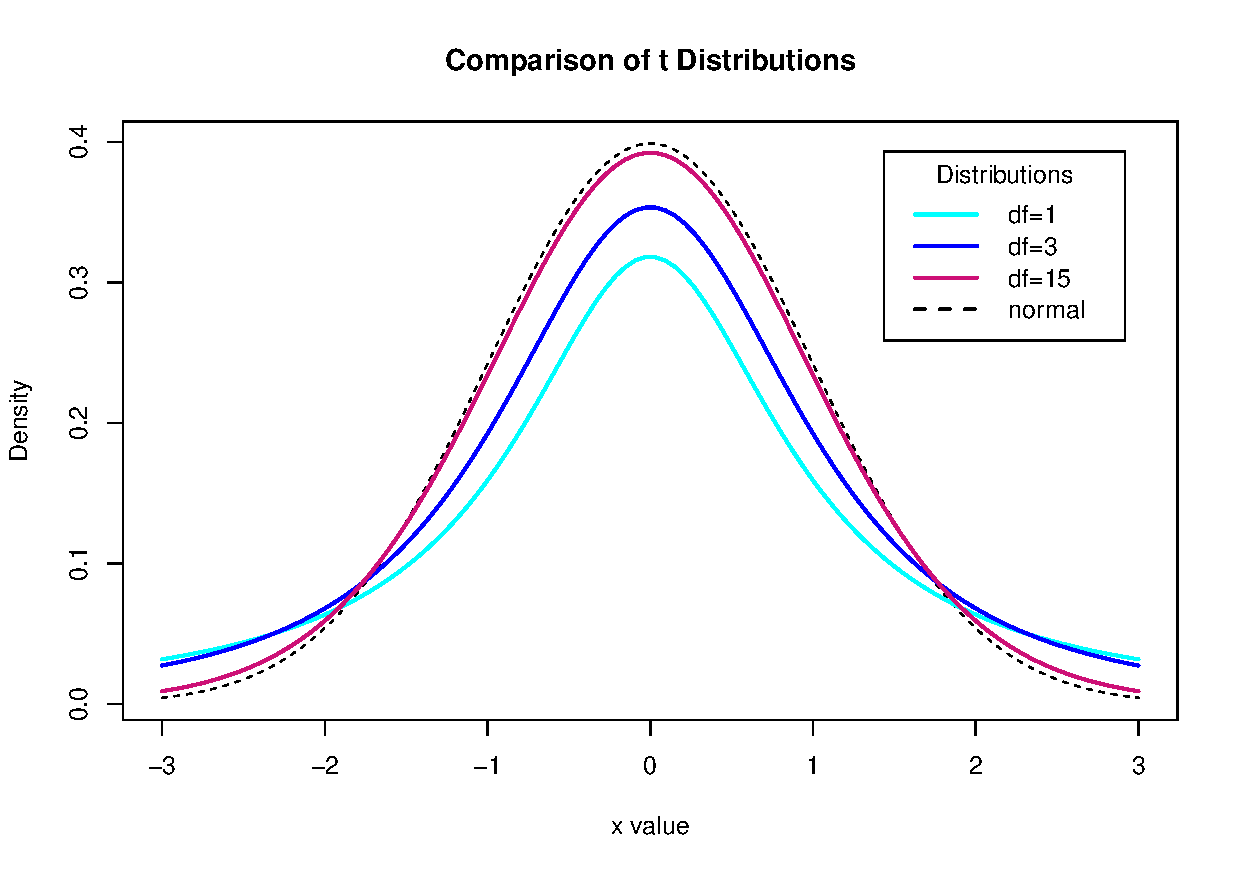
\includegraphics[width = 0.8\textwidth]{figures/t_distribution.pdf}
    \caption{The $t$-distribution for various degrees of freedom compared to the standard normal distribution.}
    \label{fig:t_distribution}
\end{figure}

Clearly, as the degrees of freedom increases, the $t$-distribution approaches the standard normal distribution, so $t(n) \rightarrow N(0,1)$ for $n\rightarrow \infty$. This also follows from the Central Limit Theorem, presented later in this chapter in theorem \ref{th:Central_limit_theorem}. 

Recall that OLS produces unbiased estimates c.f.$\!$ theorem \ref{th:unbiasedness_of_ols}, let $d_j=(\textbf{X}^\top\textbf{X})^{-1}_{jj}$ denote the $j$'th diagonal element of $(\textbf{X}^\top \textbf{X})^{-1}$, let $\hat{\beta}_j(\textbf{y})$ denote the $j$'th coordinate of the OLS estimate $\hat{\beta}(\textbf{y})$ and $\hat{\sigma}^2(\textbf{y})$ denote the usual estimate for $\sigma^2$ as in \eqref{eq:sigma_hat_2_n-k-1}.

\begin{definition} [$t$-statistic] \label{def:t-test}
    Let $\beta_{0j}$ be given and consider the hypothesis $\mathcal{H}_0 \ : \ \beta_j=\beta_{0j}$. 
    The $t$-statistic for $\mathcal{H}_0$ is then given by
\begin{align}\label{eq:t_test1}
   t_j(\textbf{y};\beta_{0j}) = \frac{\hat{\beta}_j - \beta_{0j}}{\sqrt{d_j\hat{\sigma}^2(\textbf{y})}} \quad \text{for} \quad j=0,\ldots,k
\end{align}
where large values of $|t_j(\textbf{y};\beta_{0j})|$ are critical for $\mathcal{H}_0$.
\end{definition}

In order to construct a hypothesis test, the following result is needed.

\begin{theorem} [Test of Individual Parameters] \label{th:t_distribution}
Let the situation be as in definition \ref{def:t-test}. Under $\mathcal{H}_0 \ : \ \beta_j=\beta_{0j}$ we have 
\begin{align}
   t_j(\textbf{y};\beta_{0j})  \sim t(n-k-1) \quad \text{for} \quad j=0,\ldots,k
\end{align}
and the $p$-value is
\begin{align}\label{eq:t_test_pvalue}
    p(\textbf{y},\beta_{0j})=P\Big(|t_j(\textbf{Y};\beta_{0j})|\geq |t_j(\textbf{y};\beta_{0j})|\Big).
\end{align}
The p-value is the probability that, if the null hypothesis were true, sampling variation would produce an estimate that is further away from the hypothesised parameter value than our data estimates.  
Thus it would lie in the tails of the $pdf$ of the $t$-distribution seen in figure \ref{fig:t_distribution}.
Meaning that a low $p$-value is evidence against $\mathcal{H}_0$.

Furthermore, for $0<\alpha<1$, using the $t$-test at level $\alpha$, the limits of a ($1-\alpha$)-confidence interval for $\beta_j$ is
\begin{align} \label{eq:t_statistic}
    \hat{\beta}_{j}(\textbf{y}) \pm t_{1-\alpha/2}(n-k-1)\sqrt{d_j\hat{\sigma}^2(\textbf{y})}
\end{align}
which corresponds to the cases where we accept the hypothesis that $\beta_j$ takes a specific value.
\end{theorem}
\begin{proof}
We want to verify that \eqref{eq:t_test1} has a $t$-distribution. Recall due to the assumptions \ref{as:linear_in_the_parameters}, \ref{as:no_perfect_collinearity}, \ref{as:zero_conditional_mean}, \ref{as:homoskedasticity_and_no_serial_correlation} and \ref{as:normality_of_errors} example \ref{ex:MLE_for_model} showed that

\begin{align} \label{eq:th_t_test}
    \hat{\betabold}(\textbf{Y}) \sim N_k(\betabold,\sigma^2(\textbf{X}^T\textbf{X})^{-1})
\end{align}
which entails
\begin{align*}
    &\hat{\beta}_j(\textbf{Y})\sim N(\beta_j , \sigma^2d_j) \
    \Leftrightarrow \  (\hat{\beta}_j(\textbf{Y})-\beta_j) \sim N(0,\sigma^2d_j)
\end{align*}
and standardizing is done by dividing by the standard deviation, so
\begin{align*}
    (\hat{\beta}_j(\textbf{Y})-\beta_j)/\sqrt{d_j\sigma^2} \sim N(0,1).
\end{align*}
The distribution of $s^2$ comes from \eqref{eq:sigma_hat_2_n-k-1}, so
\begin{align} \label{eq:sigma_square_of_Y}
    s^2(\textbf{y}) = \dfrac{1}{(n-k-1)}\sum_{i=1}^n \hat{\varepsilon}_i^2
\end{align}
which is a sum of squared independent normally distributed random variables and therefore
\begin{align*}
s^2(\textbf{Y}) \sim \sigma^2 \chi^2(n-k-1)/(n-k-1).    
\end{align*}
We will now show that
\begin{align*}
    (\hat{\beta}_j(\textbf{Y})-\beta_j)/\sqrt{d_j\sigma^2} \sim N(0,1) \quad \text{and} \quad s^2(\textbf{Y}) \sim \sigma^2\chi^2 (n-k-1)/(n-k-1)
\end{align*}
are independent.
The independence of $s^2(\textbf{Y})$ and $\betahat$ is seen as $\betahat$ and $\textbf{r}(\textbf{y}) = \textbf{y} -\textbf{X} \betahat$ are independent, which will be explained in detail below.
Consider
\begin{align*}
    \textbf{r}(\textbf{y}) = \textbf{y}-\textbf{X} \betahat = \textbf{y} - \textbf{H} \textbf{y} = (\textbf{I}-\textbf{H})\textbf{y} = (\textbf{I}-\textbf{H}) (\textbf{X} \betahat + \epsilonhat) = (\textbf{I} - \textbf{H}) \epsilonhat.
\end{align*}
It is seen that $E(\epsilonhat) = \textbf{0}$ by assumption \ref{as:normality_of_errors}. 
Now the expected value of the product $\textbf{r}(\textbf{y}) \betahat^\top$ is calculated, in order to later calculate the covariance
\begin{align} \label{eq:Variance_of_product}
    E(\textbf{r}(\textbf{y}) \betahat^\top) &= E \left( [(\textbf{I} - \textbf{H}) \epsilonhat] [(\textbf{X}^\top \textbf{X})^{-1} \textbf{X}^\top \textbf{y}]^\top \right) \nonumber \\
    &= E \left( [(\textbf{I}-\textbf{H}) \epsilonhat] \textbf{y}^\top \textbf{X} (\textbf{X}^\top \textbf{X})^{-1} \right) \nonumber \\
    &= (\textbf{I}-\textbf{H}) E(\epsilonhat \textbf{y}^\top ) \textbf{X}(\textbf{X}^\top \textbf{X})^{-1}. 
\end{align}
For clarity we take out the term $E(\epsilonhat \textbf{y}^\top )$ and calculate it separately
\begin{align*}
    E \left[ \epsilonhat \textbf{y}^\top \right] &= E \left[ \epsilonhat (\epsilonhat^\top + \betahat^\top \textbf{X}^\top) \right] \\
    &= E \left[ \epsilonhat \epsilonhat^\top + \epsilonhat \betahat^\top \textbf{X}^\top \right] \\
    &= E[\epsilonhat \epsilonhat^\top]
\end{align*}
This is equal to the variance of $\epsilonhat$ since $\var(\epsilonhat) = E(\epsilonhat \epsilonhat^\top) - E(\epsilonhat)E(\epsilonhat)^\top$, where $E(\epsilonhat)=\textbf{0}$.
This is by assumption \ref{as:normality_of_errors} equal to $\sigma^2 \textbf{I}_n$.
Inserting this into \eqref{eq:Variance_of_product} yields
\begin{align*}
    \sigma^2 (\textbf{I}-\textbf{H}) \textbf{X} (\textbf{X}^\top \textbf{X})^{-1} = \textbf{0}
\end{align*}
because
\begin{align*}
    (\textbf{I}-\textbf{H})\textbf{X} &= (\textbf{I}-\textbf{X}(\textbf{X}^\top \textbf{X})^{-1}\textbf{X}^\top)\textbf{X} \\
    &= \textbf{X} - \textbf{X} (\textbf{X}^\top \textbf{X})^{-1} (\textbf{X}^\top \textbf{X}) \\
    &= \textbf{X} - \textbf{X} = \textbf{0}
\end{align*}
Therefore the covariance and by extension correlation is
\begin{align*}
    \cov (\betahat, \textbf{r}(\textbf{y})) &= E(\betahat\textbf{r}(\textbf{y})^\top) - E(\betahat) E(\textbf{r}(\textbf{y}))^\top \\
    &= \textbf{0} - E(\betahat) \cdot \textbf{0}
\end{align*}
Assuming that they are multivariate normally distributed, this means that $\betahat$ and $s^2(\textbf{Y})$ are independent, since $s^2(\textbf{Y})$ is just a constant times $SSR$ c.f.$\!$ \eqref{eq:sigma_square_of_Y}.

We see that
\begin{align*}
    \frac{s^2(\textbf{Y})}{\sigma^2(\textbf{Y})} \sim \chi^2(n-k-1)/(n-k-1)
\end{align*}
and with use of definition \ref{def:t_distribution} we obtain that
\begin{align*}
    t_j(\textbf{Y};\beta_j)=\frac{(\hat{\beta}_j(\textbf{Y})-\beta_j)/\sqrt{d_j\sigma^2(\textbf{Y})}}{\sqrt{d_js^2(\textbf{Y})/d_j\sigma^2}} \sim t(n-k-1)
\end{align*}
and hence the first part of the theorem composed of \eqref{eq:th_t_test} is verified, and second part follows immediately. 
\end{proof}

In the case of testing OLS estimates, we usually test the special case where the estimates are anything other than zero. In this case, we test against the two-tailed alternatives and therefore the primary interest is testing the null hypothesis
\begin{align} \label{eq:t_test_h0}
    \mathcal{H}_0:\beta_j=0.
\end{align}
In this case the alternative hypothesis is
\begin{align} \label{eq:t_test_ha}
    \mathcal{H}_1 : \beta_j \neq 0,
\end{align}
which means, that $\textbf{x}_j$'s effect on the expected value $\textbf{y}$ can be both positive or negative.
Since after controlling for all other independent variables than $\textbf{x}_j$, $\beta_j$ measures the partial effect of $\textbf{x}_j$ on the expected value of $\textbf{y}$. 
Thus \eqref{eq:t_test_h0} means that, after $\textbf{x}_1,\textbf{x}_2, \ldots, \textbf{x}_{j-1}, \textbf{x}_{j+1}, \ldots, \textbf{x}_k$ have been accounted for, $\textbf{x}_j$ has no effect on the expected value for $\textbf{y}$ since $\beta_j=0$. 
For $\textbf{x}_j$ having a partial effect on the expected value of $\textbf{y}$, the value of $\beta_j$ has to be anything other than zero.

In practice, $\hat{\beta}_j$ will rarely be zero, whether or not $\mathcal{H}_0$ is true.
Therefore the question is rather how to determine how far $\hat{\beta}_j$ is from zero. 
The further the sample value of $\hat{\beta}_j$ is from zero, the bigger is the evidence against $\mathcal{H}_0$. 
However, the larger the standard error is of $\hat{\beta}_j$, the smaller is the evidence against $\mathcal{H}_0$. 
Thus $t_{j}$ is a ratio of how many estimated standard deviations $\hat{\beta}_j$ is away from zero.
In general the larger value of $t_{j}$, the larger the evidence against $\mathcal{H}_0$. 
The precise rule for rejecting $\mathcal{H}_0$ depends on the alternative hypothesis and the chosen significance level.
The $t$-value in \eqref{eq:t_statistic} is found using the inverse of the \textit{cdf} of the $t$-distribution with $(n - k - 1)$ degrees of freedom evaluated in $(1-\alpha/2)$. 
Since the $t$-distribution is symmetric, $\pm t_{1-\alpha/2}$ is the same as $\mp t_{\alpha/2}$.

\subsubsection{Application of \textit{t}-test}  \label{ex:ttest}
Consider the simple model with one independent variable for each of the cities 
\begin{align*}
    \log(price) \sim \log(size).
\end{align*}
The test is two-tailed, therefore we test the null hypothesis $\mathcal{H}_0:\beta_1=0.$
We complete the $t$-test at significance level $\alpha=0.05$ which gives the limits of a 95\%-confidence interval for $\hat{\beta}_1$.
We obtain the estimated model for Copenhagen with values listed in the following table.

\begin{table}[H]
\centering
\begin{tabular}{lrrrr}
\toprule
\textbf{term} & \textbf{estimate} & \textbf{std.error} & \textbf{t value} & \textbf{p.value}\\
\midrule
(Intercept) & 10.52852 & 0.07412 & 142.05 & <2e-16\\
$\log(size)$ & 0.96832 & 0.01682 & 57.59 & <2e-16\\
\bottomrule
\end{tabular}
\caption{Summary for the regression $\log(price) \sim \log(size)$ for Copenhagen.}
\end{table}

In order to calculate the $t$-value of $\hat{\beta}_1$ we define the values in \eqref{eq:t_test1}:
\begin{lstlisting}
#We define some useful values according to our definition and theorem
n <- 1182 ; k <- 1
beta_hat <- 0.96832 ; beta_null <- 0
df <- n - (k + 1)
x <- c(rep(1, n), log(Copenhagen$size)); X <- matrix(data = x, nrow = n)
y <- c(log(Copenhagen$price))
d <- solve((t(X) %*% X)) ; d_j <- d[2,2]
fitted <- X %*% solve(t(X) %*% X) %*% t(X) %*% y
sigma_hat2 <- sum((y - fitted)^2)/(n-2)
std_error <- (sqrt(d_j*sigma_hat2))
\end{lstlisting}
Now we can calculate the $t$-value by inserting the obtained values in \eqref{eq:t_test1}.
\begin{lstlisting}
#t-statistic
t_stat <- (beta_hat-beta_null)/std_error; t_stat
[1] 57.58523
\end{lstlisting}
and the p value by inserting the obtained values in \eqref{eq:t_test_pvalue}.
\begin{lstlisting}
#p-value
p_val <- pt(t_stat, df = df, lower.tail = FALSE)*2; p_val
[1] 0
\end{lstlisting}
The parameter $\hat{\beta}_1=0.96832$ has $t$-value $t_1 = 57.58523$ which is significant because of the low $p$-value. 
Therefore we reject the null hypothesis at a $5\%$-significance level. 
This is illustrated in figure \ref{fig:t_distributionplot1}, where the dotted lines illustrates the respective end and beginning of the the rejection regions.
In the figure it is clear, that we are far into the tail of the null distribution which also indicates a small $p$-value. 
This indicates, that our observed $\hat{\beta}_1$ is more extreme than what is reasonably expected if the null hypothesis were true.
\begin{figure}[H]
    \centering
    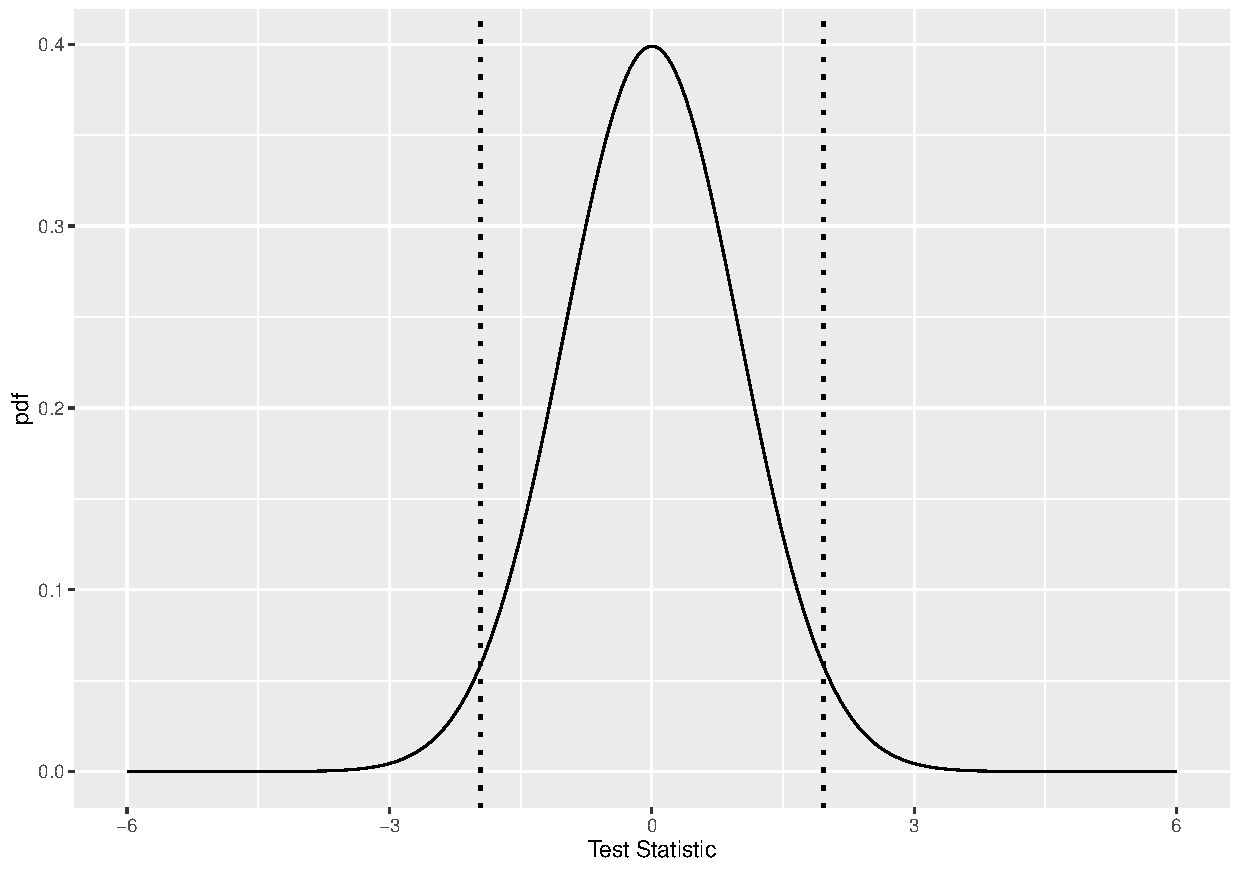
\includegraphics[width = 0.6  \textwidth]{figures/Nanna/t_distribution123.pdf}
    \caption{5 \% rejection rule for $\mathcal{H}_1:\beta_1\neq0$ with 1180 degrees of freedom. The $t$ value of the observed value $\hat{\beta}_1=0.96832$ is far out in the tail to the right.}
    \label{fig:t_distributionplot1}
\end{figure}
The critical $t$-values for $\mathcal{H}_0$ is found by the inverse of the $cdf$ where we obtain the $t$-values of chosen probabilities. 
The $95\%$-significance level, means that we evaluate the inverse $cdf$ in $0.025$ and $0.975$. 
This is illustrated in figure \ref{fig:CDF_inverse} where the intersection of the dotted lines gives the critical $t$-values.
\begin{figure}[H]
    \centering
    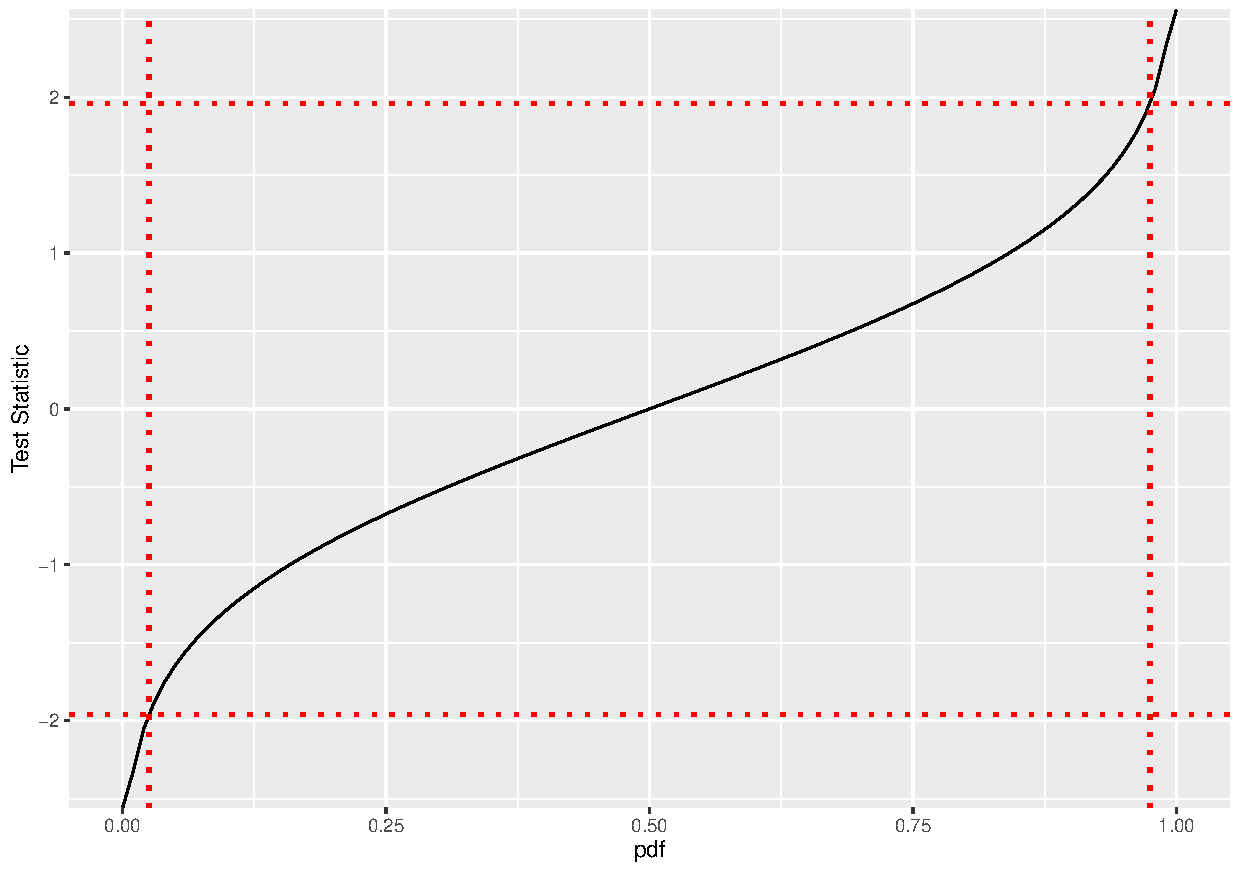
\includegraphics[width = 0.5\textwidth]{figures/Nanna/Inverse_CDF.pdf}
    \caption{The inverse $cdf$ in which we obtain the critic values for $\mathcal{H}_0$ of the chosen $95\%$-significance level.}
    \label{fig:CDF_inverse}
\end{figure}
Now we have concluded, that $\log(size)$ has a statistically significant effect on $\log(price)$ at a 95\%-confidence level for Copenhagen. 
By computing the limits of a 95\%-confidence interval for $\hat{\beta}_1$ with \eqref{eq:t_statistic}, we find the 95\%-confidence interval which we expect contains the ``true'' parameter.
\begin{lstlisting}
#We calculate the confidence interval for our parameter
beta_hat+std_error*qt(0.975, df = df)
[1] 1.001311
beta_hat+std_error*qt(0.025, df = df)
[1] 0.9353285
\end{lstlisting}
Note that the confidence interval for $\betahat_1$ does not contain 0, as expected.
From this lower and upper bound of the confidence intervals of the parameters, we can plot the area in which we expect the ``true'' line to be. 
In figure \ref{fig:t_distributionplot2} the blue line is our estimated model and the shaded area is the 95\%-confidence interval of the model. 
\begin{figure}[H]
    \centering
    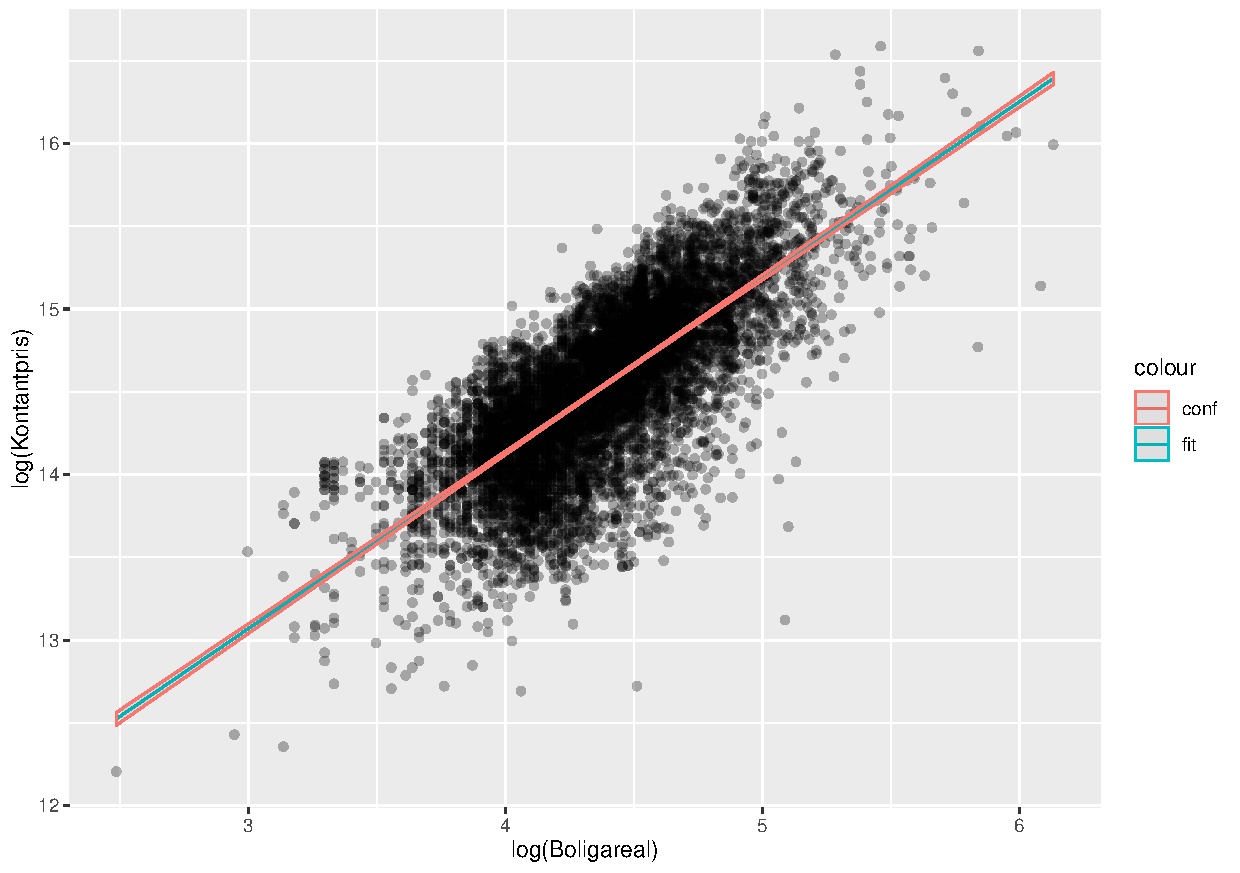
\includegraphics[width = 0.7\textwidth]{figures/Nanna/Confidence_interval.pdf}
    \caption{Plot of the observed values, the fitted regression line and its $95\%$-confidence intervals in which we expect the ``true'' line to be.}
    \label{fig:t_distributionplot2}
\end{figure}

For the remaining cities, we draw the same conclusions. 
Each of the simple models of the cities gives $t$-statistics that entails significant $p$-values and we can reject the null hypothesis in all cases. 
Therefore, we conclude that $\log(size)$ has a statistically significant effect on $\log(price)$ at a 95\%-confidence level in Copenhagen, Aarhus, Odense and Aalborg. 

We have performed $t$-test for each of the parameters presented in section \ref{sec:modelling} for each of the four cities. As a result, \textit{balcony} and \textit{year.sale} are also significant for each of the four cities. 
Varying results are obtained for the remaining parameters, which indicates, that different parameters determine the price for each city. The parameter \textit{cond} is also significant for Copenhagen but only for the value ``high''. 

From the $t$-test, we have obtained knowledge of the parameters individual effect on $\log(price)$ and if the effect is considered as significant. 
In order to test models with more than one parameter, we therefore introduce the $F$-test as a method.

% \section{Confidence intervals}

% \begin{definition} [The (1-$\alpha$)-confidence Region]
% \label{def:confidence_region}
% Suppose that for a given number $\alpha \in (0,1)$ and for each $\textbf{y} \in \mathcal{Y}$, we have specified a subset $A(\textbf{y})$ of the parameter space $\Theta^k$, such that
% \begin{align*}
%     P_{\boldsymbol{\beta}} (\boldsymbol{\beta} \in A(\textbf{Y})) = 1 - a, \quad \forall \boldsymbol{\beta} \in \Theta^k
% \end{align*}
% Then we call $A(y)$ a $(1-\alpha)$-confidence region for $\boldsymbol{\beta}$.
% \end{definition}

% If the parameter is one-dimensional $(k=1)$ and the observations, $y$ are normally distributed, then the confidence region become the interval

% \begin{align*}
%     \left[ 
%     \hat{\beta}(\textbf{y}) + \Phi_{\alpha/2} \sqrt{D(\hat{\beta}(\textbf{y})} , \hat{\beta}(\textbf{y}) + \Phi_{1 - \alpha/2} \sqrt{D(\hat{\beta}(\textbf{y})}
%     \right]
% \end{align*}

% for $0 < \alpha \leq 0.5$. 


% \begin{example}
% Consider again the situation from example \ref{ex:model1}. By theorem \ref{th:distribution_ml_estimator} the asymptotic distribution of the ML estimator is given by
% \begin{align*}
%     \betahat \rightarrow^\mathcal{D} N\left( \mathbf{ \beta }, \boldsymbol{i}(\betahat)^{-1} \right)
% \end{align*}
% Since $\mathbf{\beta}$ is one-dimensional, $k=1$, and for $0\leq \alpha \leq 0.5$ we have the approximate $(1-\alpha)$-confidence interval
% \begin{align*}
% \left[ \betahat(\mathbf{y}) + \Phi_{\alpha/2} \sqrt{D\left( \betahat\left(\mathbf{y}\right)\right)}, \betahat(\mathbf{y}) + \Phi_{1 - \alpha/2} \sqrt{D\left( \betahat\left(\mathbf{y}\right)\right)} \right],
% \end{align*}
% where $D\left(\betahat(\mathbf{y})\right) = j\left(\betahat(\mathbf{y})\right)^{-1}$.
% For $\alpha=0.05$ we have the approximate $95\%$-confidence interval for $\mathbf{\beta}$:
% \begin{align*}
% \left[ \bar{y} - \frac{1.96}{\sqrt{n}}, \bar{y} + \frac{1.96}{\sqrt{n}} \right]    
% \end{align*}
% \end{example}

\subsection{F-Test}\label{sec:Ftest}
Suppose we want to test if a multiple regression model has redundant explanatory variables.
In terms of hypothesis testing this is the null hypothesis: A set of variables has no statistically significant effect on $\textbf{y}$, once another set of variables has been controlled for.

Determining this will be done by analyzing the change in $SSR$, that is the difference in how well the models explain the variation in the data, and determining whether this change is significant. 
Suppose we have $model$ 1 with $(k+1)$ variables 
\begin{align*}
    \textbf{y} = \textbf{X}\betabold +\ \boldsymbol{\varepsilon},
\end{align*}
this is known as the unrestricted model. The restricted model or $model$ 0 lacks the $q$ variables, for which we want to check significance, that is
\begin{align*}
    \textbf{y} = \beta_0 + \beta_1 \textbf{x}_1 + \cdots + \beta_{k-q} \textbf{x}_{k-q} + \boldsymbol{\varepsilon}.
\end{align*}
Therefore $q$ is the difference in degrees of freedom between the two models.
This means we want to test the hypothesis
\begin{align}
    \mathcal{H}_0: \beta_{k-q+1} = \ldots = \beta_k = 0.
\end{align}
These are referred to as the exclusion restrictions. 
This is done using the $F$-statistic
\begin{align}\label{eq:F_statistic}
    F \equiv \frac{\| \textbf{H}_1 \textbf{y} - \textbf{H}_0 \textbf{y} \|^2/q}{\| \textbf{y} - \textbf{H}_1 \textbf{y} \|^2/(n-k-1)},
\end{align}
that is the relative increase in $SSR$, when going from $model$ 0 to $model$ 1. 
$\| \textbf{y} - \textbf{H}_0 \textbf{y} \|^2$ is the $SSR$ of $model$ 0 and $\| \textbf{y} - \textbf{H}_1 \textbf{y} \|^2$ is that of $model$ 1. 
$q$ is referred to as the numerator degrees of freedom, and $(n-k-1)$ is the denominator degrees of freedom. 

The change in $SSR$, when going from $model$ 0 to $model$ 1, is always non-negative because the model has more parameters to explain the data. 
This is discussed further in theorem \ref{th:Likelihood_ratio_linear_models}.

We will therefore reject $\mathcal{H}_0$, when $F$ is sufficiently large compared to the critical value, since this indicates that significantly more of the variation of the data has been explained by $model$ 1, as compared to $model$ 0.

As with the $t$-test, there is no correct significance level, but $\alpha = 0.05$ is often chosen. 
The critical value for the significance level can be determined by calculating one explicitly from the $cdf$ of the $F$-distribution found below see definition \ref{def:F-distribution}. 
This is equivalent to the procedure for $t$-test.

$\mathcal{H}_0$ is therefore rejected if the $F$-statistic is greater than the critical value
\begin{align*}
    F>c.
\end{align*}
If this is the case, the explanatory variables $\textbf{x}_{k-q+1}, \ldots, \textbf{x}_k$ are said to be jointly statistically significant. 
Otherwise they are said to be jointly insignificant, which can justify removing them from the model. 
In order to determine the critical value, the $F$-distribution is given.
\begin{definition}[$F$-Distribution]\label{def:F-distribution}
    Let $X_1 \sim \chi_{k_1}^2$ and $X_2 \sim \chi_{k_2}^2$ be independent random variables. Then the random variable 
        \begin{align*}
            F(k_1,k_2) = \frac{X_1/k_1}{X_2/k_2}
        \end{align*}
    has an $F$-distribution with $(k_1, k_2)$ degrees of freedom, which is denoted as $F(k_1,k_2) \sim F_{k_1, k_2}$.
\end{definition}
The $p$-value for the $F$-test is analogouse to that of the $t$-test
\begin{align*}
    p = P(F_{q,n-k-1} > F).
\end{align*}
That is the probability of observing this $F$-statistic under $\mathcal{H}_0$. 
The confidence level therefore reflects how sure we are that the model under $\mathcal{H}_0$ has generated the data.

\subsubsection{Equivalence of Tests}
The likelihood ratio can compare the goodness of fit for two models, specifically one over the entire parameter space and one with a restriction imposed.
It would therefore be interesting to see what relation it has to the $F$-test. 
Below it will be shown that the $F$-test is actually equivalent to the likelihood ration test.
This means that, going forward, we can just use the $F$-test to test joint significance for parameters.
Note this is only the case for multiple regression. 

\begin{theorem}[Likelihood Ratio For Linear Models]
\label{th:Likelihood_ratio_linear_models}
    The Likelihood ratio
    \begin{align*}
        \lambda(\textbf{y}) = \frac{\sup \ L(\textbf{y};\boldsymbol{\mu}_0, \sigma_0^2)}{\sup \ L(\textbf{y};\boldsymbol{\mu}_1, \sigma_1^2)}
    \end{align*}
    is a strictly decreasing function of $F(\textbf{y})$ under $\mathcal{H}_0$, such that
    \begin{align*}
        F(\textbf{Y}) \sim F_{q, n-k-1}.
    \end{align*}
\end{theorem}

\begin{proof}
    Under $\mathcal{H}_1$: $\hat{\boldsymbol{\mu}}_1 = \textbf{H}_1 \textbf{y}$ and $\hat{\sigma}_1^2 = \frac{\| \textbf{y} - \textbf{H}_1 \textbf{y} \|^2}{n}$, the log-likelihood 
    function for the normal distribution is
    \begin{align*}
        l(\textbf{y};\hat{\boldsymbol{\mu}}_1, \hat{\sigma}_1^2) &= -\frac{n}{2} log(\hat{\sigma}_1^2) - \frac{1}{2 \hat{\sigma}_1^2} \| \textbf{y} - \textbf{H}_1 \textbf{y} \|^2 \\
        &= -\frac{n}{2} log(\hat{\sigma}_1^2) - \frac{n}{2},
    \end{align*}
    and similarly for $\mathcal{H}_0$. Therefore the likelihood ratio can be written as
    \begin{align*}
        \lambda(\textbf{y}) &= \exp \left( l(\textbf{y};\hat{\boldsymbol{\mu}}_0, \hat{\sigma}_0^2) - l(\textbf{y};\hat{\boldsymbol{\mu}}_1, \hat{\sigma}_1^2) \right) \\
        &= \exp \left( -\frac{n}{2} \Big( log(\hat{\sigma}_0^2) - log(\hat{\sigma}_1^2)\Big) \right) \\
        &= \left( \frac{\| \textbf{y} - \textbf{H}_1 \textbf{y} \|^2}{\| \textbf{y} - \textbf{H}_0 \textbf{y} \|^2} \right)^{\frac{n}{2}} \\
        &= \left( \frac{\| \textbf{y} - \textbf{H}_1 \textbf{y} \|^2}{\| \textbf{y} - \textbf{H}_1 \textbf{y} \|^2 + \| \textbf{H}_1 y - \textbf{H}_0 \textbf{y} \|^2} \right)^{\frac{n}{2}}.
    \end{align*}
    The last equation holds because $\textbf{y} - \textbf{H}_1 \textbf{y}$ is orthogonal to $\Omega_1$ and $(\textbf{H}_1 \textbf{y} - \textbf{H}_0 \textbf{y}) \in \Omega_1$. 
    Dividing by the numerator and using \eqref{eq:F_statistic}, the above equation becomes
    \begin{align*}
        \lambda(\textbf{y}) &= \left( \frac{1}{1 + \frac{\| \textbf{H}_1 \textbf{y} - \textbf{H}_0 \textbf{y} \|^2}{\| \textbf{y} - \textbf{H}_1 \textbf{y} \|^2}} \right)^{\frac{n}{2}} \\
        &= \left( \frac{1}{1 + \frac{q}{n-k-1}F(\textbf{y})}  \right)^{\frac{n}{2}}.
    \end{align*}
    The likelihood ratio is therefore a function of $F$, and since it is in the denominator, $\lambda(\textbf{y})$ is a decreasing function of $F(\textbf{y})$. We again see that large values of $F$ are critical, since small values of $\lambda(\textbf{y})$ are critical.
    
    The fact that $F$ is $F$-distributed is seen from
    \begin{align*}
        F(\textbf{Y}) &= \frac{\| \textbf{H}_1 \textbf{Y} - \textbf{H}_0 \textbf{Y} \|^2/q}{\| \textbf{Y} - \textbf{H}_1 \textbf{Y} \|^2/(n-k-1)} \\
        &= \frac{\| (\textbf{H}_1 - \textbf{H}_0) \textbf{Y} \|^2/q}{\| (\textbf{I} - \textbf{H}_1) Y \|^2/(n-k-1)} \\
        &\sim \frac{\chi^2(q)/q}{\chi^2(n-k-1)/(n-k-1)}, \\
    \end{align*}
    cf. definition \ref{def:F-distribution}. Here the last equation holds because $\textbf{H}_1 - \textbf{H}_0$ and $\textbf{I} - \textbf{H}_1$ are projections and therefore follow a $\chi^2$ distribution.
\end{proof}

\begin{theorem}
    The $t$-test in \eqref{def:t-test} is equivalent to the likelihood ratio test for $\mathcal{H}_0 \ : \ \beta_j = \beta_{0j}$ since the $p$-values are the same.
\end{theorem}
\begin{proof}
    Without loss of generality assume that $j = 1$.
    Let $\betabold_{-1} = (\beta_2, \ldots, \beta_k)^\top$, so $\betabold = (\beta_1, \beta_{-1}^\top)^\top$.
    Denote by $\textbf{x}_1$, the first column of $\textbf{X}$, and by $\textbf{X}_{-1}$, the remaining columns of $\textbf{X}$, such that $\textbf{X} = \left[\textbf{x}_1 \ \textbf{X}_{-1}\right]$.
    
    Consider first the case $\beta_{01} = 0$: Then $\textbf{X}_{-1}$ is the design matrix for $\mathcal{H}_0$.
    The hat matrices corresponding to $\textbf{X}$ and $\textbf{X}_{-1}$ are given by
    \begin{align*}
        \textbf{H} = \textbf{X}(\textbf{X}^\top\textbf{X})^{-1}\textbf{X}^\top, \quad \mathbf{H}_{-1} = \textbf{X}_{-1}(\textbf{X}^\top_{-1}\textbf{X}_{-1})^{-1}\textbf{X}^\top_{-1},
    \end{align*}
    respectively.
    The MLE for the mean vector under the original model is $\textbf{H}\textbf{y}$, the MLE for the mean vector under $\mathcal{H}_0$ is $\textbf{H}_{-1}\textbf{y}$, and the $F$-statistic for $\mathcal{H}_0$ is
    \begin{align*}
        F(\textbf{y}) = \frac{\|\textbf{H}\textbf{y} - \textbf{H}_{-1}\textbf{y}\|^2/(k-(k-1))}{\hat{\sigma}^2(\textbf{y})}
    \end{align*}
    where large values of $F(\textbf{y})$ are critical for $\mathcal{H}_0$.
    We have
    \begin{align*}
        \textbf{H}\textbf{y} = \textbf{X}\betahat(\textbf{y}) = \textbf{x}_1\hat{\beta}_1(\textbf{y}) + \textbf{X}_{-1} \betahat_{-1}(\textbf{y})
    \end{align*}
    and $\textbf{H}_{-1}\textbf{H} = \textbf{H}_{-1}$, so
    \begin{align*}
        \textbf{H}\textbf{y}-\textbf{H}_{-1}\textbf{y} = 
        \textbf{H}\textbf{y}-\textbf{H}_{-1}\textbf{H}\textbf{y} =
        (\textbf{I} - \textbf{H}_{-1})\textbf{H}\textbf{y} = 
        (\textbf{I} - \textbf{H}_{-1})\textbf{x}_1\hat{\beta}_1(\textbf{y})
    \end{align*}
    since $(\textbf{I} - \textbf{H}_{-1})\textbf{X}_{-1} = 0$.
    Hence, as $\textbf{I} - \textbf{H}_{-1}$ is symmetric and idempotent,
    \begin{align*}
        \|\textbf{H}\textbf{y} - \textbf{H}_{-1}\textbf{y}\|^2 = \hat{\beta}_1(\textbf{y})^2\textbf{x}_1^\top(\textbf{I} - \textbf{H}_{-1})\textbf{x}_1.
    \end{align*}
    In appendix \ref{ch:block_matrix_inversion} it is verified that $\textbf{x}_1^\top(\textbf{I} - \textbf{H}_{-1})\textbf{x}_1 = 1/d_1$.
    Consequently,
    \begin{align*}
        F(\textbf{y}) = \frac{\hat{\beta}(\textbf{y})^2/d_1}{\hat{\sigma}^2(\textbf{y})} = t_1(\textbf{y};0)^2
    \end{align*}
    and so the $t$-test in theorem (specify which) is equivalent to the $F$-test, in the case of $df=1$, which in turn is equivalent to the likelihood ratio test.
    
    Consider next the general case where $\beta_{01}$ is any fixed number: Let $\textbf{Z} = \textbf{Y} - \textbf{x}_1\beta_{01}$ and
    \begin{align*}
        \Tilde{\betabold} = (\beta_1 - \beta_{01}, \beta_2, \ldots, \beta_k)^\top = \betabold - (\beta_{01}, 0, \ldots, 0)^\top.
    \end{align*}
    Since $\textbf{Z} \sim N_n(\textbf{X}\Tilde{\boldsymbol{\beta}}, \sigma^2\textbf{I}_n)$ and $\{ (\beta_1 - \beta_{01}, \beta_2, \ldots, \beta_k)^\top \ : \ \beta_1 \in \mathbb{R}, \ldots, \beta_k \in \mathbb{R} \} = \mathbb{R}^k$, we see that $\textbf{Z}$ corresponds to $\textbf{Y}$ in the first case.
    It is easily seen that
    \begin{align*}
        \hat{\sigma}^2(\textbf{Z}) = \hat{\sigma}^2(\textbf{Y}), \quad \hat{\tilde{\boldsymbol{\beta}}}(\textbf{Z}) = \hat{\boldsymbol{\beta}}(\textbf{Y}) - (\beta_{01}, 0, \ldots, 0)^\top,
    \end{align*}
    since the MLE is invariant under reparametrizations and under one-to-one transformations of the data.
    Combining these facts we obtain
    \begin{align*}
        F(\textbf{z}) =
        \frac{\hat{\tilde{\boldsymbol{\beta}}}(\textbf{Z})^2/d_1}{\hat{\sigma}^2(\textbf{z})} = 
        \frac{(\betahat(\textbf{y}) - \beta_{01})^2/d_1}{\hat{\sigma}^2(\textbf{y})}
    \end{align*}
    which completes the proof.
\end{proof}

Note that the $F$-test and $t$-test are only equivalent for simple linear regression, that is $df = 1$, since the $t$-statistic only checks significance for one parameter.

In practice it can be useful to express the $F$-statistic as a function of $R$-squared instead of $SSR$, as it can become large, making computation slower, whereas $R$-squared is always between $0$ and $1$. In addition many programs often report $R$-squared and not $SSR$.

This form of the $F$-statistic is obtained by using the equality's $SSR_0 = SST(1 - R^2_0)$ and $SSR_1 = SST(1-R^2_1)$. Substituting these into \eqref{eq:F_statistic} yields
\begin{align}\label{eq:F_test_R}
    F &= \frac{(SST(1 - R^2_0) - SST(1-R^2_1)/q}{SST(1-R^2_1)/(n-k-1)} \nonumber \\
    F &= \frac{(R^2_1 - R^2_0)/q}{(1 - R^2_1)/(n-k-1)}.
\end{align}


\subsubsection{Application of \textit{F}-test}\label{sec:app_F_test}
This subsection will use the F-test to compare the full model from section \ref{sec:modelling}, to a model containing the parameters with highest R-squared. 
The intuition here is that \textit{log(size)} and \textit{year.sale} explain much more of the variation than \textit{balcony} and \textit{cond} do.
Additionally this subsection will also evaluate other models constructed from the parameters discussed in section \ref{sec:modelling}.
% As seen above we only need the degrees of freedom in order to find the $F$-distribution and thereby the critical value, for a given significance level.
Firstly our models are introduced
\begin{lstlisting}
# The Models
linreg1 <- lm(log(price) ~ log(size) + year.sale + cond + balcony, 
    data = cities.data)
linreg0 <- lm(log(price) ~ log(size) + year.sale, data = cities.data)
    
# Degrees of freedom
n <- length(cities.data$price)
dfmod1 <- n - length(linreg1$coefficients)
dfmod0 <- n - length(linreg0$coefficients)
\end{lstlisting}
Here the dataset cities.data containing only observations for Copenhagen is used.
The $pdf$ for our $F$-distribution is then found using the \texttt{df} function in R, not to be confused with the degrees of freedom. 
\begin{lstlisting}
dist_df <- data.frame(
x = seq(0.8, 1.2, by = 0.001),
pdf = df(x = seq(0.8, 1.2, 0.001), df1 = dfmod1, df2 = dfmod0)
)
\end{lstlisting}
We choose a significance level of $\alpha = 0.05$, from which we get the critical value $c=1.10142$. 
This is found using the quantile function
\begin{lstlisting}
upper = qf(0.95, df1 = dfmod1, df2 = dfmod0)
\end{lstlisting}
The $pdf$ and associated critical value are now plotted
    
\begin{lstlisting}
ggplot(aes(x = x, y = pdf), data = dist_df) +
geom_line()
# Mark significance level
geom_area(data=dist[which(dist$x > upper),], aes(x=x, y=pdf), 
fill = "red", alpha = 0.6)
\end{lstlisting}
    
\begin{figure}[H]
    \centering
  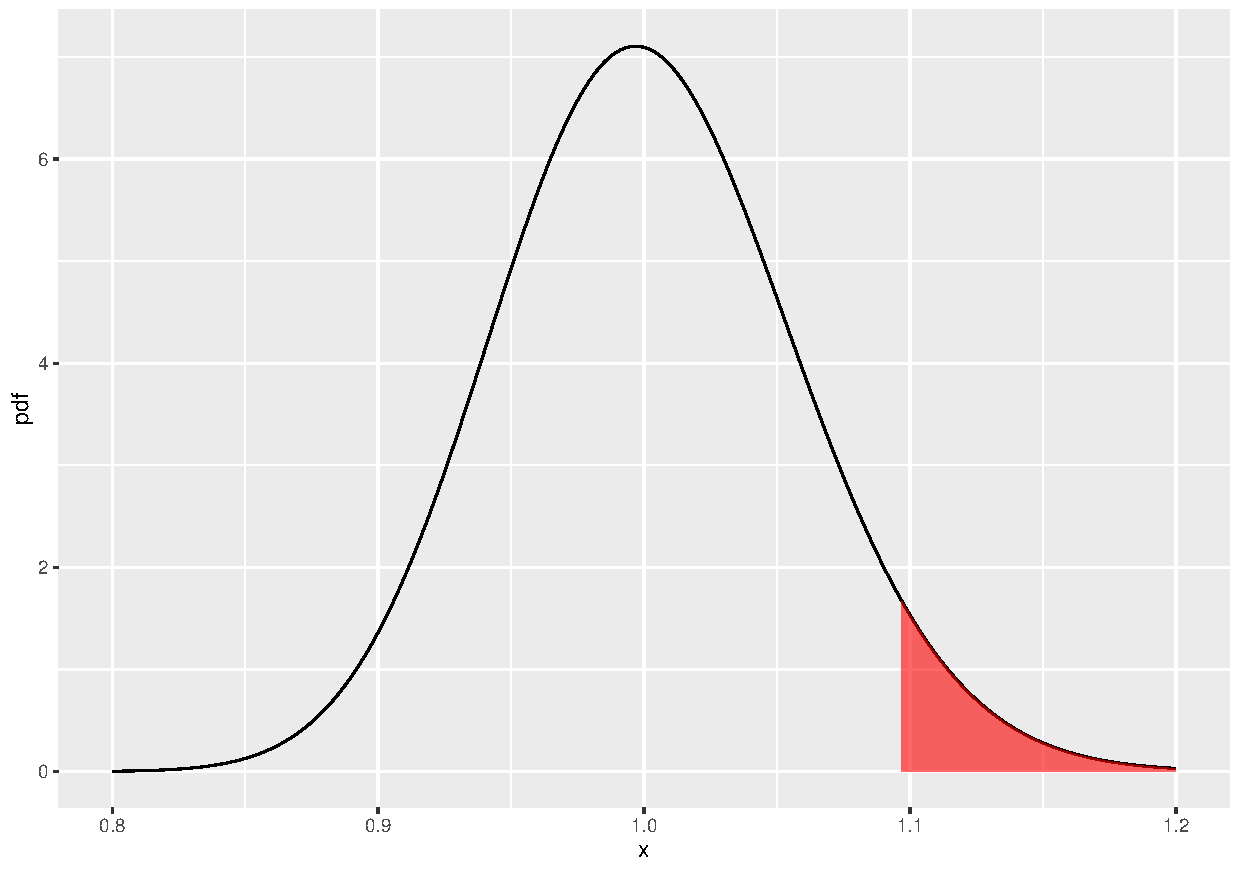
\includegraphics[width = 0.5 \textwidth]{figures/Fdistsign.pdf}
  \caption{Pdf for F-distribution with significance level}
  \label{fig:my_label}
\end{figure}
    
The significance level is illustrated by the area under the curve marked with red, and has area equal to the significance level.
Note that the $pdf$ converges toward a normal distribution, as the degrees of freedom increases.
    
The $F$-statistic is calculated using \eqref{eq:F_statistic}, where the $SSR$ for the two models are calculated by the \texttt{anova} function in R. 
%Kode til Fstat
\begin{lstlisting}
# Residuals
RSS_model1 <- anova(linreg1,linreg0)$RSS[1]; RSS_model1
24.10871
RSS_model0 <- anova(linreg1,linreg0)$RSS[2]; RSS_model0
28.50651
# F-statistic
Fstat <- ((RSS_model0 - RSS_model1)/(dfmod0 - dfmod1))/
((RSS_model1)/(dfmod1)); Fstat
43.67925
\end{lstlisting}
The associated $p$-value is then
\begin{lstlisting}
p <- pf(q = Fstat, df1 = dfmod0, df2 = dfmod1, lower.tail = F)
<2.2e^{-16}
\end{lstlisting}
or effectively zero. We therefore conclude that the additional parameters are statistically significant.
It may seem as though any parameter would be significant, but this is because of our initial filtering and large dataset.
The filtering done in section \ref{sec:modelling} removed parameters with poor fit, thereby only leaving likely significant parameters.
In addition the large dataset also plays a role, since the difference in degrees of freedom is relatively small for many observations. 
This does not mean that the full model is a lot better, since the additional 2 parameters only explain about $9\%$ of the remaining residuals. 

This test was done using only observations from Copenhagen and performing the same procedure for the observations from Aalborg gives $F=0.7301$ and $p=0.5345$.
Meaning that the full model is not significantly better than one containing only $log(size)$ and $year.sale$, when only considering observation from Aalborg.

Alternatively we could check all possible combinations of parameters, to see if any of the the corresponding models contain statistically insignificant parameters.
In order to avoid testing all possible combination it would be beneficial, to determine which parameter adds the least fit to the model and then remove the variables in that order. 

% Choosing the order of which to remove the parameters is known as subset selection and there are several different approaches.
% One method is called backwards step wise selection. 
% The approach is to first remove the parameter that explains the least variation in the data, in order to remove the parameters in a strategic manner.
% More specifically it is a greedy algorithm that starts with the full model, and at each step removes the parameter which adds the least to the $R$-squared.

Backwards selection is used to chose the order of which to remove the parameters.
In table \ref{tbl:backward_order_of_parameters} the order of parameters removal is listed for each of the cities.
    
\begin{table}[H]
    \centering
    \begin{tabular}{r|llll}
        \toprule
        \textbf{Order} & \textbf{Copenhagen} & \textbf{Aarhus} & \textbf{Odense} & \textbf{Aalborg}\\
        \midrule
        1 & $balcony$              & $balcony$         & $cond$            & $cond$ \\
        2 & $cond$           & $cond$            & $balcony$         & $balcony$ \\
        3 & $year.sale$    & $year.sale$  & $year.sale$  & $year.sale$ \\
        4 & $log(size)$         & $log(size)$       & $log(size)$       & $log(size)$ \\
        \bottomrule
    \end{tabular}
    \caption{The order of which backwards stepwise selection removes the parameters for each of the cities.}
    \label{tbl:backward_order_of_parameters}
\end{table}

Using this to compare the full model to one with one removed, we notably get a $p$-value of 0.2944 for Aarhus, 0.3943 for Odense and 0.5025 for Aalborg. 
In the same manner we find the second removed parameter for Aalborg to also be insignificant with a p-value of 0.3678, as expected from the first test.
This means that the following models have significant parameters.
\begin{align*}
    log(price)_{Cph.F} &\sim log(size) + year.sale + cond + balcony \\
    log(price)_{Aar.F} &\sim log(size) + year.sale + cond \\
    log(price)_{Ode.F} &\sim log(size) + year.sale + balcony \\
    log(price)_{Aal.F} &\sim log(size) + year.sale \\
\end{align*}
The F-test only takes the available data into account and can not test how well it aligns with new observations.
It therefore does not measure how good these models are at predicting future apartment prices, and only validates the model based on previouse observations. 



% This means that the model, containing the parameter \textit{selling.period}, is not significantly improved compared to the one without this parameter.
% Comparing the remaining models, we find that all other parameters significantly improves the models. 
% The decision of whether or not to include the additional parameters, then becomes a trade off between better model fit and potential overfitting.
% This will be explored further in the next section.
    
    
    
    % The reason they are still significant is because the decrease in degrees of freedom is relatively small, due to the large set of observations.
    % The $F$-test is therefore best suited for smaller datasets, and we will now look at another way to validate models based on a larger amount of observations. 

\section{Cross-Validation} \label{sec:CV}

Previously we applied the $F$-statistic for the purpose of testing whether or not the model should be restricted. 
As we concluded in section \ref{sec:Ftest}, the $F$-test is more suitable for datasets of fewer observations. 
This is the motivation for using cross validation in order to test the selected variables and the models performance.
Cross-validation is a widely used method for estimating prediction error.
There are many variations of cross-validation, and this project will only cover a limited selection. 

\subsection{\textit{K}-Fold Cross-Validation} 

This method uses part of the data to fit the model and another to test it. This is done via the following process.

The data is split up in $K$ partitions, where one of them is retained as the test or validation fold. 
The remaining $K-1$ partitions are referred to as training sets and are used to fit the model.
This process is repeated $K$ times, where each partition is used as the validation set once. 
This way the entire dataset is used, while keeping the modelling and validation data separate. 

More formally, let $\kappa: \{1, \ldots, n\} \rightarrow \{1, \ldots, K\}$ be the function that indicates which partition observation $i$ belongs to. 
Denote the model fitted with the $k$'th part of the data removed by $(\textbf{x}_i \betahat)^{-\kappa(i)}$. 
Then the cross-validation estimate of the prediction error, for the $k$'th fold, is 
\begin{align*}
    CV(\betahat)_k = \frac{1}{n} \sum_{i=1}^n L\left(y_i, (\textbf{x}_i \betahat)^{-\kappa(i)}\right),
\end{align*}
where we choose the loss function $L\left(y_i, (\textbf{x}_i \betahat)^{-\kappa(i)}\right)=\left(y_i - (\textbf{x}_i \betahat)^{-\kappa(i)}\right)^2$, which indicates how much of the variation in the data is explained by the model fitted from the subset that did not include the $k$'th partition. 

A common choice is $K = 5$, which is what we will use in this project. 
The case $K = n$ is known as leave-one-out cross-validation. 
This tests every possible combination, that is $\kappa(i) = i$. 
This method is approximately unbiased, since each training set is comparatively small, but since the training sets are so similar the variance may be greater. 
Conversely $K=5$ has lower variance, as each training partition is larger, but bias may be a problem. 


\subsection{Application of \textit{K}-fold Cross-Validation}
%Modelselection - forward
In order to test the effect of each parameter, they need to be added one by one. 
% Choosing the order to add the parameters is known as subset selection and there are several different approaches.
We use forward step wise selection to choose the order. The intuition behind this method is:
We want to first add the parameter that individually explains the most variation in the data, in order to end up with the best possible model after having removed some of the parameters.
Here best refers to the model that increases $R$-squared the most.
% More specifically it is a greedy algorithm that starts with the intercept, and at each step adds the parameter with the highest $R$-squared.

After performing the forward stepwise selection on the four cities the order of which the parameters are added can be seen in table \ref{tbl:order_of_parameters}.
To give a little explanation of the table, suppose we want a model considering Aalborg with 2 parameters.
We then choose the Aalborg column and go down to the second row of the table, and see that the model would be on the form $log(price) \sim \log(size) + year.construct$.
\begin{table}[H]
    \centering
    \begin{tabular}{r|llll}
        \toprule
        \textbf{Order} & \textbf{Copenhagen} & \textbf{Aarhus} & \textbf{Odense} & \textbf{Aalborg}\\
        \midrule
        1 & $\log(size)$        & $\log(size)$      & $\log(size)$      & $\log(size)$ \\
        2 & $year.sale$         & $year.sale$       & $year.sale$       & $year.sale$ \\
        3 & $cond$    & $cond$  & $balcony$  & $cond$ \\
        4 & $balcony$           & $balcony$            & $cond$         & $balcony$ \\
        \bottomrule
    \end{tabular}
    \caption{The order of which forward stepwise selection adds the parameters for each of the cities.}
    \label{tbl:order_of_parameters}
\end{table}
%\textbf{TOMMELFINGERREGEL}
%Knowing this, we can make sure that we omit the parameter that contributes least to R-squared first, and thereby achieving the best model. 
%Using this model we now move on to applying cross-validation. 

In figure \ref{fig:CrossValidationCopenhagen} cross-validation is performed for the HOME dataset that only contains the observations for Copenhagen.
For each fold the prediction error (RMSE) has been plotted for each of the six models from table \ref{tbl:order_of_parameters}. Every fold gives varying predictions errors for each model which indicates some randomness crosswise the five folds. The model with the lowest RMSE therefore differs depending on the selected train and testset. 
Thus the interesting result is the meanplot in which the standard errors are calculated for the five folds.
Clearly, the models with most variation crosswise the 5 folds have the highest standard errors. 

To determine the desired number of parameters, the ``one-standard-error'' rule is used. 
This states that we choose the most parsimonious model whose prediction error is no more than one standard error above the prediction error of the best model. The rule is applied to reduce the probability of overfitting and it is therefore expected, that it performs better out-of-sample. Which seems relatively fair, since the increasing in the prediction error is relatively small.

    \begin{figure}[H]
        \centering
      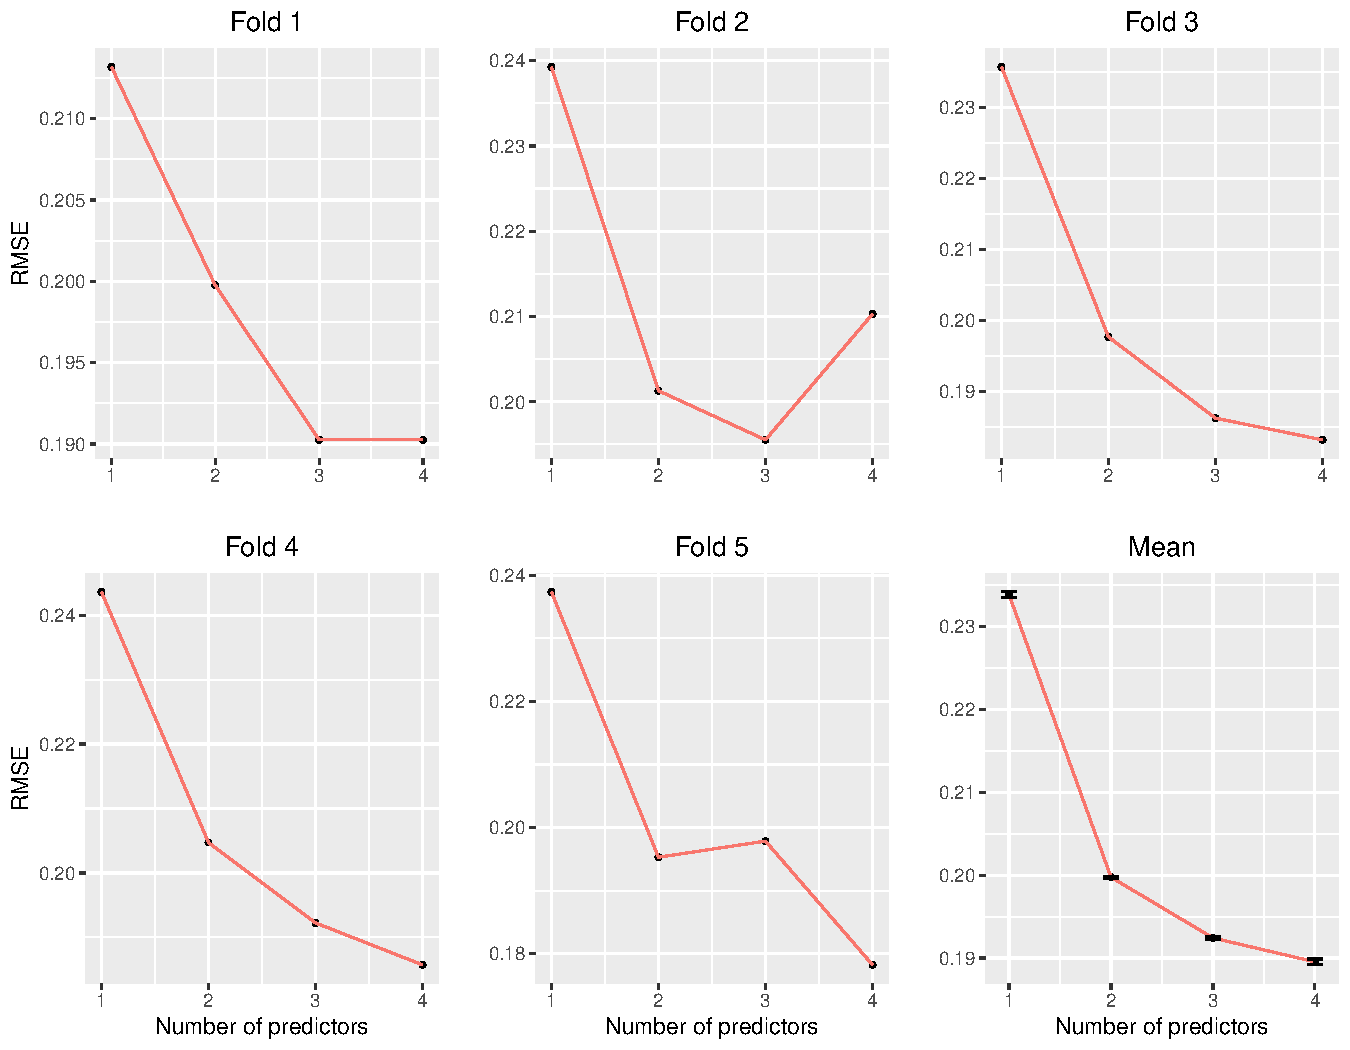
\includegraphics[width = 1 \textwidth]{figures/Nanna/CrossValidationCopenhagen.pdf}
      \caption{Plots of the prediction errors for each fold and their mean with the associated standard errors where the x-axis denotes the number of predictors in the given model.}
      \label{fig:CrossValidationCopenhagen}
    \end{figure}
    
In the case of Copenhagen observe that a model with four parameters has the lowest prediction error, then we choose the smallest number of predictors with a prediction error within the standard error for the model with four parameters.
In this case the optimal number of parameters, according to the rule, is three.

This procedure is performed for the remaining three cities. Note in table \ref{tbl:order_of_parameters} the order of the selected parameters from the execution of the forward-selection-algorithm differs between the cities. 
In figure \ref{fig:CrossValidationSamlet} is the meanplot for each city, in which we conclude from the 5-fold cross-validation, that the optimal number of parameters is three for Aarhus, one for Odense and two forAalborg.

\begin{figure}[H]
    \centering
  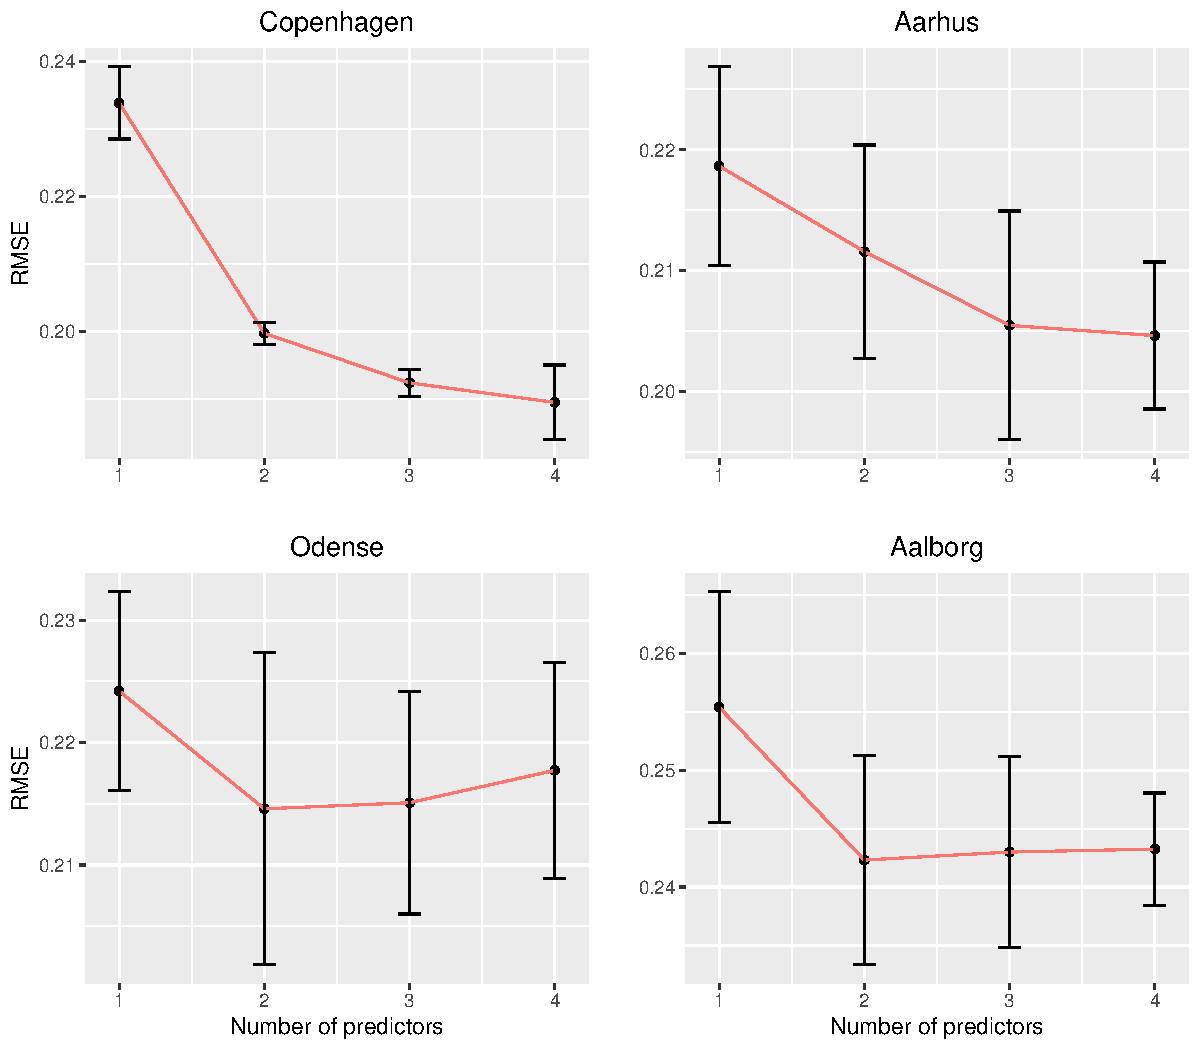
\includegraphics[width = 1 \textwidth]{figures/Nanna/CrossValidationSamlet.pdf}
  \caption{Mean plot for each city with prediction error for each model with associated standard error.}
  \label{fig:CrossValidationSamlet}
\end{figure}

The final models obtained from the result of performing 5-fold cross-validation is listed in appendix \ref{aap:cv} and is listed as follows
\begin{align*}
    log(price)_{Cph.CV} &\sim log(size) + year.sale + cond \\
    log(price)_{Aar.CV} &\sim log(size) + year.sale + cond\\
    log(price)_{Ode.CV} &\sim log(size) \\
    log(price)_{Aal.CV} &\sim log(size) + year.sale \\
\end{align*}
Due to the later purpose of testing the model on out-of-sample performance regarding predicting prices for houses sold in 2016, it is interesting to investigate the out-of-sample performance on the selected models from CV.
If the errors fulfil the earlier stated assumptions regarding normally distributed errors with mean zero and \homo, when we expect the model to perform well out-of-sample. In figure \ref{fig:cv_normal_homo} the errors obtained from the CV of Copenhagen are presented.

\begin{figure}[H]
\centering
\begin{subfigure}[b]{0.5\textwidth}
    \centering
    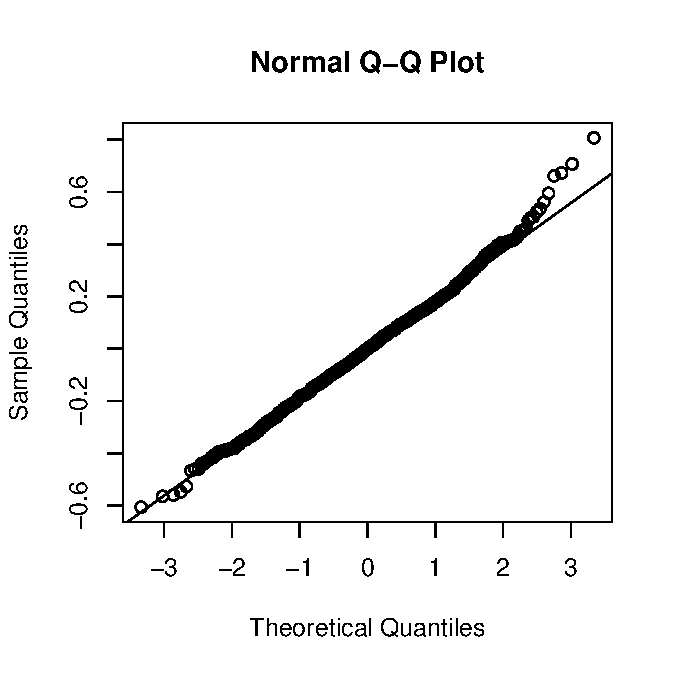
\includegraphics[width = \textwidth]{figures/Nanna/Normal.pdf}
    \caption{Testing for normality}
    \label{fig:cv_normal}
\end{subfigure}%
\begin{subfigure}[b]{0.5\textwidth}
\centering
    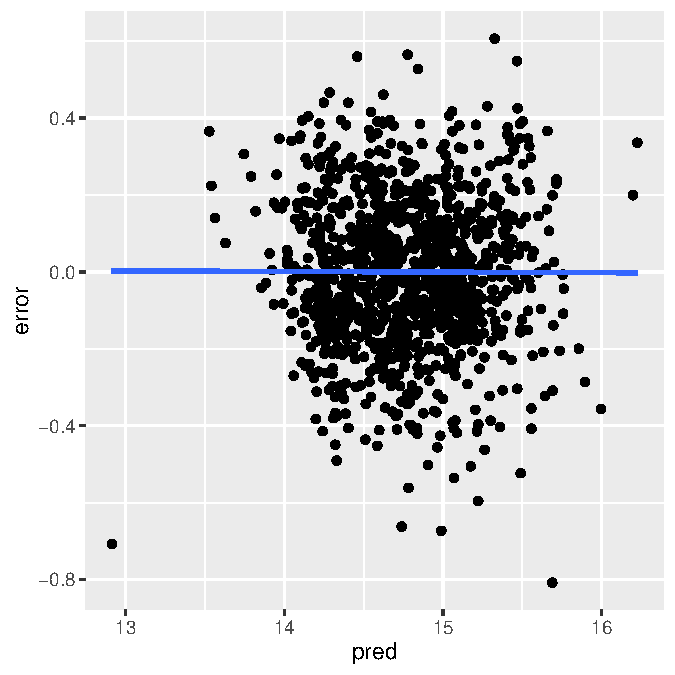
\includegraphics[width = \textwidth]{figures/Nanna/cv_normal_homo.pdf}
    \caption{Testing for \hetero}
    \label{fig:cv_homo}
\end{subfigure}
\caption{Examination of the prediction errors from the 5-fold cross validation.}
\label{fig:cv_normal_homo}
\end{figure}

From figure \ref{fig:cv_normal} it is concluded that there are problems in the tails of the errors. 
In the tails there are deviations from what is expected of the normal distribution. 
This might cause problems with both the confidence and prediction interval of the model, since this does not take the larger tails into account.
The tails indicates, that the intervals should be enlarged.
Therefore, the model is now suspected to have some difficulties performing out-of-sample. 
In figure \ref{fig:cv_homo} the errors seems overall homoskedastic with mean zero. 

\section{Residuals}\label{subsec:residuals}
So far we have only discussed residuals in passing. 
This chapter will therefore present different types of residuals and their properties.
Residuals are the difference between the observed values $\textbf{y}$ and the fitted values $\hat{\textbf{y}}$. They are therefore the errors $\boldsymbol{\hat{\varepsilon}}$ described in \eqref{eq:replace_with_y}
\begin{align*}
    \textbf{r}(\textbf{y}) &= \textbf{y} - \hat{\textbf{y}} = \textbf{y} - \textbf{X} \betahat = (\textbf{I} - \textbf{H}) \textbf{y}.
    % r_i(y) &= y_i - x_i \betahat = y_i - x_i (X^\top X)^{-1}X^\top y_i = (1 - h_{ii}) y_i,
\end{align*}
By assumption \ref{as:normality_of_errors} the residuals have variance
\begin{align*}
    Var(\textbf{r}(\textbf{Y})) &= \sigma^2 (\textbf{I} - \textbf{H}) \\
    Var(r_i(\textbf{Y})) &= \sigma^2(1 - h_{ii}),
\end{align*}
where $h_{ii}$ is the $i$'th diagonal element in $\textbf{H}$. The second equation follows, since the first equation is just the variance-covariance matrix for the residuals, which has variances in the diagonal.
Rewriting \eqref{eq:sigma_hat_2_n-k-1} using projection matrices gives the following estimate for the parameter variance
\begin{align*}
    \hat{\sigma}^2(\textbf{Y}) &= \frac{\| \textbf{Y} - \textbf{X} \betahat (\textbf{y}) \|^2 }{n-k-1} = \frac{\| \textbf{Y} - \textbf{H} \textbf{Y} \|^2}{n-k-1} .
\end{align*}
Residuals can be used to identify outliers, which is the observations that do not fit the general pattern of the data.
These data points can have a large effect on the estimated variance and it would therefore be useful to have a way to measure how much variance an observation adds.
We use the notation $-i$, which refers to the removal of the $i$'th row e.g.
\begin{align*}
    \textbf{y}_{-i} = (y_1, \ldots, y_{i-1}, y_{i+1}, \ldots, y_n)^\top.
\end{align*}
The estimate for $\sigma^2$ found by deleting the $i$'th row is then
\begin{align*}
    \hat{\sigma}^2_{-i}(\textbf{Y}) = \frac{\| \textbf{Y}_{-i} - \textbf{H}_{-i} \textbf{Y}_{-i} \|^2}{n-1-(k+1)}.
\end{align*}
We now introduce the studentized residual $(\textbf{r}^{rt})$, which takes into account the variance without the i'th observation, thereby giving a more accurate measure of the standard deviation
\begin{align*}
    r_i^{rt} = \frac{r_i}{\sqrt{\hat{\sigma}^2_{-i}(1-h_{ii})}}.
\end{align*}
If this value in deemed to high, it should be investigated and could potentially justify removing it as an outlier/measurement error. We now introduce an important property of the studentized residuals.

\begin{proposition}
    Consider a general linear model $\textbf{Y} \sim N_n(\textbf{X} \betabold, \sigma^2 \textbf{I}_n)$ where the design matrix has full rank $k \leq n-3$ and $\textbf{H} = \textbf{X} (\textbf{X}^\top \textbf{X})^{-1}\textbf{X}^\top$ is the corresponding projection-matrix, then
    \begin{align*}
        r_i^{rt}(\textbf{Y}) \sim t(n-k-2).
    \end{align*}
\end{proposition}
\begin{proof}
    Without loss of generality let $i=1$. 
    To summarize the above results
    \begin{align*}
        r_1^{rt}(\textbf{Y}) = \frac{r_1(\textbf{Y})}{\sqrt{\hat{\sigma}^2_{-1}(\textbf{Y}_{-1})(1-h_{11})}}
        =
        \frac{r_1(\textbf{Y})/ \sqrt{\sigma^2 (1-h_{11})}}{\sqrt{\hat{\sigma}_{-i}^2 (\textbf{Y}_{-1})/\sigma^2}},
    \end{align*}
    which has the distribution
    \begin{align*}
        \frac{N(0,1)}{\sqrt{\chi^2(n-k-2)/(n-k-2)}} = t(n-k-2)
    \end{align*}
    Therefore we just need to prove that they are independent.
    Using the definition of the residual $r_1(\textbf{Y}) = Y_1 -  (\textbf{HY})_1$ and the projection matrix
    \begin{align*}
        \begin{bmatrix}
            r_1(\textbf{Y}) \\
            \textbf{Y}_{-1} - \textbf{H}_{-1} \textbf{Y}_{-1}
        \end{bmatrix}
        =
        \begin{bmatrix}
            Y_1 - \textbf{x}_1^\top (\textbf{X}^\top \textbf{X})^{-1} \textbf{X}^\top \textbf{Y} \\
            \textbf{Y}_{-1} - \textbf{X}_{-1} (\textbf{X}_{-1}^\top \textbf{X}_{-1})^{-1} \textbf{X}_{-1}^\top \textbf{Y}_{-1}
        \end{bmatrix}
    \end{align*}
    This can be written as the matrix-vector product
    \begin{align*}
        \begin{bmatrix}
            1 - \textbf{x}_1^\top (\textbf{X}^\top \textbf{X})^{-1} \textbf{x}_1^\top & - \textbf{x}_1^\top (\textbf{X}^\top \textbf{X})^{-1} \textbf{X}_{-1}^\top \\
            \textbf{0} & \textbf{I}_{n-1} - \textbf{X}_{-1} (\textbf{X}_{-1}^\top \textbf{X}_{-1})^{-1} \textbf{X}_{-1}^\top
        \end{bmatrix}
        \begin{bmatrix}
            Y_1 \\
            \textbf{Y}_{-1}
        \end{bmatrix}
        =
        \textbf{AY} =
                \begin{bmatrix}
            \textbf{A}_1 \\
            \textbf{A}_2
        \end{bmatrix}
        \textbf{Y}
        \sim N(\cdot)
              \
    \end{align*}
    Therefore $\textbf{A}_1 \textbf{Y} = r_1(\textbf{Y})$ and $\textbf{A}_2 \textbf{Y} = \textbf{Y}_{-1} - \textbf{H}_{-1} \textbf{Y}_{-1}$ are independent if they are uncorrelated. Their covariance matrix is given by 
    \begin{align*}
        \cov(\textbf{A}_1 \textbf{Y}, \mathbf{A}_2 \textbf{Y}) &= \textbf{A}_1\  \var(\textbf{Y}) \ \textbf{A}_2^\top = \textbf{A}_1 \sigma^2 \textbf{I}_n \textbf{A}_2^\top = \sigma^2 \textbf{A}_1 \mathbf{A}_2^\top \\
        &= \sigma^2 
        \begin{bmatrix}
            1 - \textbf{x}_1^\top (\textbf{X}^\top \textbf{X})^{-1} \textbf{x}_1^\top & - \textbf{x}_1^\top (\textbf{X}^\top \textbf{X})^{-1} \textbf{X}_{-1}^\top
        \end{bmatrix}
        \cdot
        \begin{bmatrix}
            \textbf{0}^\top \\
            \textbf{I}_{n-1} - \textbf{X}_{-1} (\textbf{X}_{-1}^\top \textbf{X}_{-1})^{-1} \textbf{X}_{-1}^\top
        \end{bmatrix} \\
        &= \sigma^2 (- \textbf{x}_1^\top (\textbf{X}^\top \textbf{X})^{-1} \textbf{X}_{-1}^\top) (\textbf{I}_{n-1} - \textbf{X}_{-1} (\textbf{X}_{-1}^\top \textbf{X}_{-1})^{-1} \textbf{X}_{-1}^\top) \\
        &= \sigma^2 (- \textbf{x}_1^\top (\textbf{X}^\top \textbf{X})^{-1} \textbf{X}_{-1}^\top + \textbf{x}_1^\top (\textbf{X}^\top \textbf{X})^{-1} \textbf{X}_{-1}^\top \textbf{X}_{-1} (\textbf{X}_{-1}^\top \textbf{X}_{-1})^{-1} \textbf{X}_{-1}^\top) \\
        &= \sigma^2 (- \textbf{x}_1^\top (\textbf{X}^\top \textbf{X})^{-1} \textbf{X}_{-1}^\top + \textbf{x}_1^\top (\textbf{X}^\top \textbf{X})^{-1} \textbf{X}_{-1}^\top) \\
        &= \textbf{0},
    \end{align*}
    and therefore uncorrelated and because they are jointly normally distributed also independent.
\end{proof}

The distribution of the studentized residuals should therefore be checked, in order to verify assumption \ref{as:normality_of_errors}. 
Since the $t$-distribution converges toward the normal distribution for large datasets, a plot similar to \ref{fig:studentized_res_plot} is often made.

\subsection{Application of Studentized Residuals} \label{sub:residuals}

In this application we want to verify the earlier stated assumption \ref{as:normality_of_errors} about the errors for the models obtained from the $F$-test and from the 5-fold cross-validation. 
Since the error term is unobserved, the investigation is performed on the residuals of the models.
Odense is the illustrated case in figure \ref{fig:studentized_res_plot}, since only Aarhus and Odense have different results from the $F$-test compared to cross-validation.

Both models seem to comply well with assumption \ref{as:normality_of_errors}, and are almost exactly the same.
Both have more data located at the left tail of the distribution, as compared to the normal distribution. 
This means there are more large negative errors than expected, which is obviously undesirable for a model used for prediction. 
This is only a problem for a small part of the dataset, and the model may therefore still be good as a rough estimate. 
As a result, we expect that the 95\% prediction interval and the 95\% confidence interval of the models should be larger, given that these are calculated for the normal distribution.

\begin{figure}[H]
    \centering
  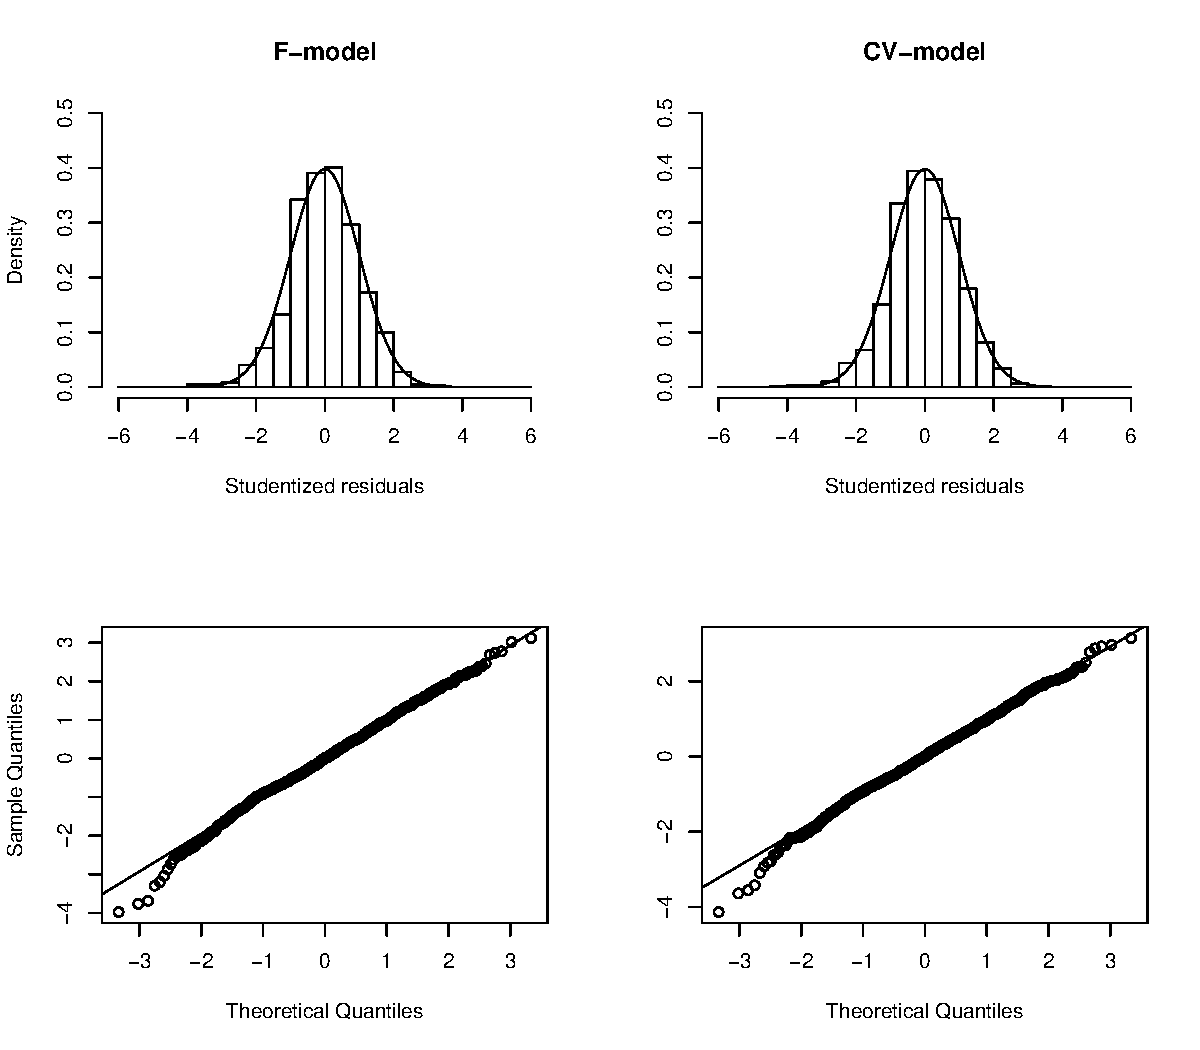
\includegraphics[width = 0.9 \textwidth]{figures/Nanna/studentized_res_plot.pdf}
  \caption{QQ-plot and histogram plot for the studentized residuals for the F-model and CV-model respectively for Copenhagen.}
  \label{fig:studentized_res_plot}
\end{figure}

For Aarhus the model obtained from cross-validations seems to satisfy the stated assumptions slightly better than the model obtained from the $F$-test. 
For Odense and Aalborg the residuals are approximately normal distributed. 
However, the residuals of the model for Aalborg differs the most from a normal distribution, as illustrated in figure \ref{fig:studentized_res_plot_Aalborg}.
Therefore, we expect the Aalborg model to have slightly inferior predictive performance compared to the other models.

\begin{figure}[H]
    \centering
  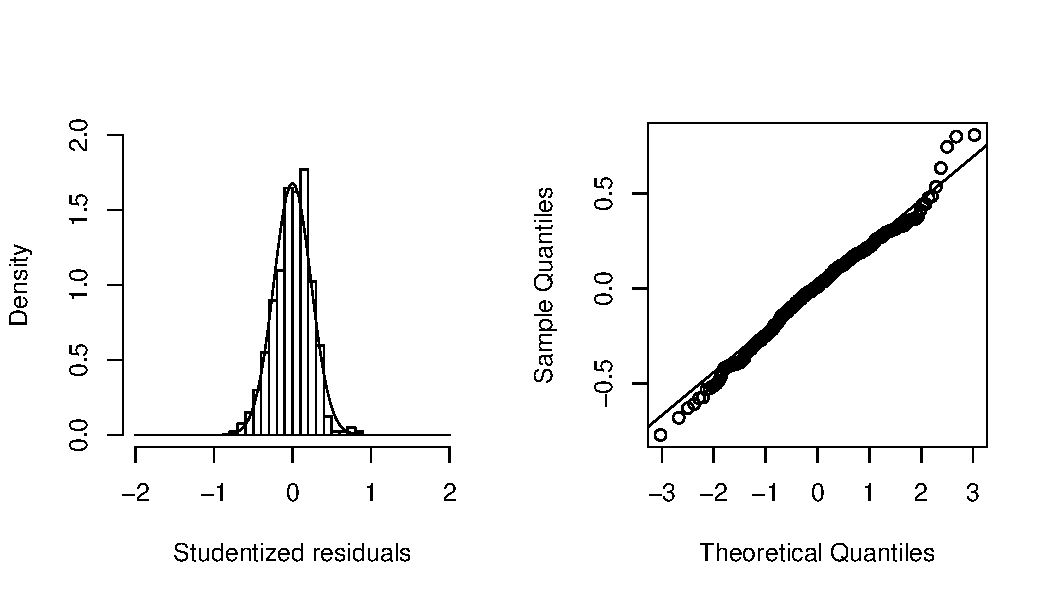
\includegraphics[width = 0.95 \textwidth]{figures/Nanna/NormalAal.pdf}
  \caption{QQ-plot and histogram plot for the studentized residuals using observation from Aalborg.}
  \label{fig:studentized_res_plot_Aalborg}
\end{figure}

% The same data as in section ?? is used
% \begin{lstlisting}
%     #The studentized residuals are found for each model
%     res1 <- rstudent(mod1)
%     res2 <- rstudent(mod2)
    
%     #Histogram for the residuals, and associated normal distribution
%     hist(res1,prob=TRUE); curve(dnorm(x,mean(res1),sd(res1)),add=TRUE)
%     hist(res2,prob=TRUE); curve(dnorm(x,mean(res2),sd(res2)),add=TRUE)
% \end{lstlisting}
% The residuals for both models clearly follow a normal distribution and assumption \ref{as:normality_of_errors} is therefore satisfied, as illustrated in figure \ref{fig:studentized_res_plot}.
%     \begin{figure}[H]
%         \centering
%       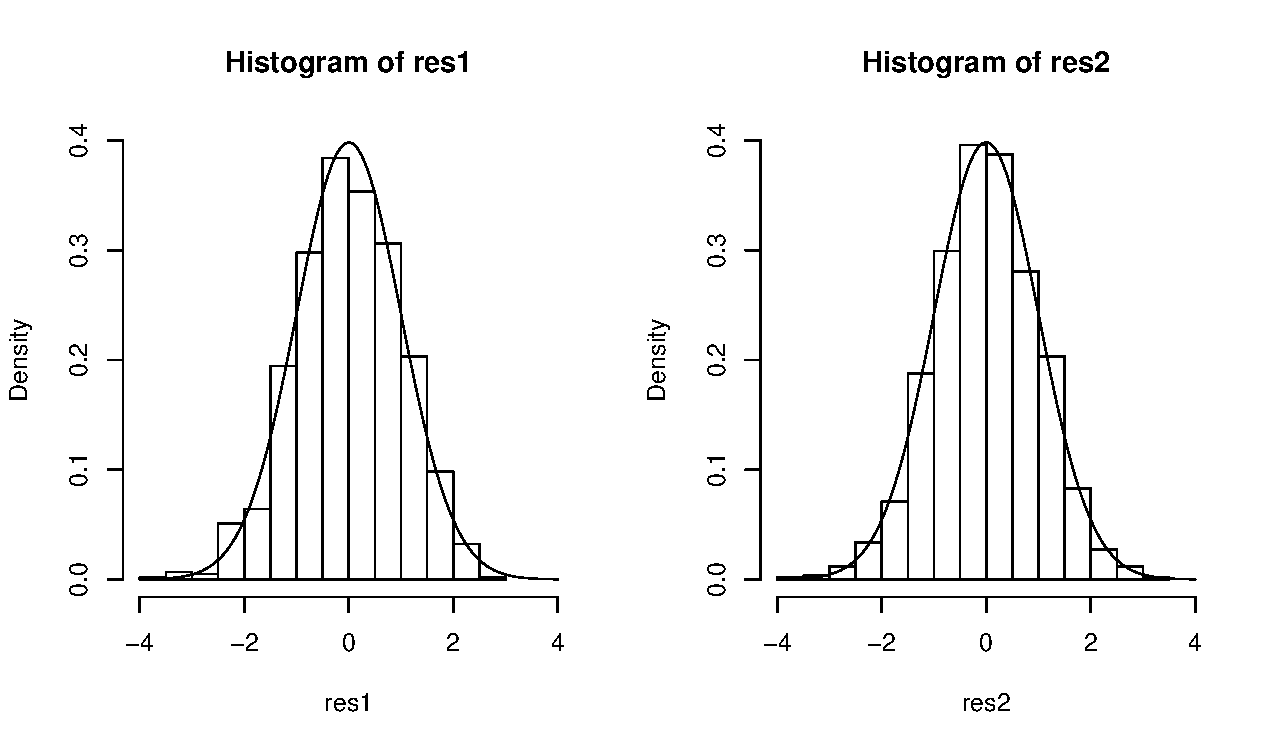
\includegraphics[width = 1 \textwidth]{RRESIUDALPLOT_HISTOGRAM.pdf}
%       \caption{Distribution of Studentized Residuals.}
%       \label{fig:studentized_res_plot}
%     \end{figure}


\section{Testing and Correcting for Heteroskedasticity}
In this section we wish to introduce methods for detecting heteroskedasticity and afterwards how to correct for heteroskedasticity so it is possible to test hypotheses when evaluating our models in the case of heteroskedasticity.

\subsection{Test for Heteroskedasticity}
In this section we wish to introduce a method to determine if heteroskedasticity is present, because in the case of heteroskedasticity the usual OLS estimator is not BLUE c.f.$\!$ \ref{as:homoskedasticity_and_no_serial_correlation}. 

We consider our linear model given as $\textbf{y} = \textbf{X} \betabold + \boldsymbol{\varepsilon}$ and let assumption \ref{as:linear_in_the_parameters}, \ref{as:no_perfect_collinearity} and \ref{as:zero_conditional_mean} hold. We then construct our null hypothesis as
\begin{align*}
    \mathcal{H}_0 : \var[\boldsymbol{\varepsilon} | \mathbf{X}] = \var[\boldsymbol{\varepsilon}] = \sigma^2 \textbf{I}_n. 
\end{align*}
With this null hypothesis we wish to determine if the homoskedasticity assumption holds true. 
If we accept our $\mathcal{H}_0$-hypothesis for a small significance level, then heteroskedasticity is with a high probability not present.
Assumption \ref{as:zero_conditional_mean}, which says that the conditional expected value of $\boldsymbol{\varepsilon}$ is equal to $\textbf{0}$, implies that $\var(\boldsymbol{\varepsilon} | \mathbf{X}) = E[\boldsymbol{\varepsilon \varepsilon^\top} | \mathbf{X}]$ because of the conditional variance formula $\var(\boldsymbol{\varepsilon} | \mathbf{X}) = E[\boldsymbol{\varepsilon \varepsilon^\top} | \mathbf{X}] - E[\boldsymbol{\varepsilon} | \mathbf{X}]E[\boldsymbol{\varepsilon}^\top | \mathbf{X}]$. 
Using this we rewrite our $\mathcal{H}_0$-hypothesis as
\begin{align*}
    \mathcal{H}_0 : E[\boldsymbol{\varepsilon \varepsilon^\top} | \mathbf{X}] = E[\boldsymbol{\varepsilon \varepsilon^\top}] = \sigma^2\textbf{I}_n.
\end{align*}
With this $\mathcal{H}_0$-hypothesis we test if the error term, $\sigma^2$ is related with any of the explanatory variables in terms of the expected value.  
If $\mathcal{H}_0$ is rejected then $\sigma^2_i$ is a function of at least one of the explanatory variables, so the error term can be expressed as a linear function of these explanatory variables
\begin{align}\label{eq:test_hetero_nul_hypotese}
    \sigma_i^2 = \delta_0 + \delta_1x_{i,1} + \ldots + \delta_kx_{i,k} + v_i
\end{align}
where $v_i$ is an error with mean equal to $0$ given the explanatory variables. In order for $\sigma_i^2$ to be homoskedastic the following $\mathcal{H}_0$-hypothesis must be accepted 
\begin{align}\label{eq:H_nul_for_hetero_med_delta}
    \mathcal{H}_0 : \delta_1 = \delta_2 = \ldots = \delta_k = 0.
\end{align}
So the error term $\textbf{v}$ does not depend on the explanatory variables. 
If the error $v_i$ is assumed to be independent of the explanatory variables $\mathbf{X}$, then the $F$-statistics can be used to test \eqref{eq:H_nul_for_hetero_med_delta} for the overall significance of the explanatory variables for $\sigma^2$, even though this error term is not normally distributed. This is shown by the Central Limit Theorem, which we state without proof. 
\begin{theorem}[Central Limit Theorem] \label{th:Central_limit_theorem}
Let $S_n = \{ Y_1, Y_2, \ldots, Y_n \}$ be an i.i.d.$\!$ random sample with mean $\mu$ and variance $\sigma^2 < \infty$. Then
\begin{align} \label{eq:bakergud}
    P\left(\dfrac{S_n - n\mu}{\sigma \sqrt{n}}\leq y\right) \rightarrow \Phi(y)
\end{align}
where $\Phi(y)$ is the cdf of the standard normal distribution and $S_n$ is the sum of $Y$. 
\end{theorem}
From the central limit theorem it is possible to derive the distribution of $S_n$. 
We have equation \eqref{eq:bakergud} and for large $n$ we use the central limit theorem to rewrite as
\begin{align*}
    Z_n = \dfrac{S_n - n\mu}{\sigma \sqrt{n}} \stackrel{d}{\sim} N(0,1). 
\end{align*}
Where $\stackrel{d}{\sim}$ denotes the approximate distribution. It is seen that $S_n$ has mean $n\mu$ and variance $n \sigma^2$ from the above equation. We use this to write
\begin{align*}
    S_n \stackrel{d}{\sim} N(n\mu, n\sigma^2). 
\end{align*}
This means that the sum of i.i.d. random variables $S_n$ have an approximately normal distribution regardless of how $Y$ is distributed. Therefore an $F$-test for $\sigma_i^2$ is asymptotically true even though $\sigma_i^2$ is not normally distributed.  




Since $\sigma^2_i$ is unobserved we cannot calculate the OLS regression on $\sigma_i^2$ for $\mathbf{X}$, so instead we calculate the regressions using the estimates. Thus
% \begin{align}\label{eq:OLS_residual_hat_epsioln_i_anden}
%     \hat{\boldsymbol{\varepsilon}}\hat{\boldsymbol{\varepsilon}}^\top = \delta_0\textbf{1} + \delta_1\textbf{x}_1 + \ldots + \delta_k\textbf{x}_k + \mathbf{w}
% \end{align}
\begin{align}\label{eq:OLS_residual_hat_epsioln_i_anden}
    s_i^2 = \delta_0 + \delta_1x_{i,1} + \ldots + \delta_kx_{i,k} + w_i,
\end{align}
where $s^2_i$ is an estimate for $\sigma^2_i$ and $w_i$ has mean 0. From this equation the $F$-statistics for the joint significance of $\textbf{x}_1, \textbf{x}_2, \ldots, \textbf{x}_k$ can be calculated to test for multicollinearity.

In addition to section \ref{sec:Ftest} the $F$-statistic can be used to test for the overall significance of a regression. 
Consider the model with $k$ independent variables, to which the null hypothesis can be written as
\begin{align}\label{eq:null_hypo_for_F_overall_significance_R}
    \mathcal{H}_0: \beta_1 = \beta_2 = \ldots = \beta_k = 0.
\end{align}
Where the alternative hypothesis is that at least one estimator is non-zero. In \eqref{eq:null_hypo_for_F_overall_significance_R} there are $k$ restrictions and they state that knowing the values of the explanatory variables does not explain the dependent variable $y$. This can be written as
\begin{align}\label{eq:unrestricted_F_hypo_for_jeg_skal_bruge_den}
    y_i = \beta_0 + \varepsilon_i.
\end{align}
Where all independent variables have been excluded due to no effect on $y$. 
Recall equation \eqref{eq:F_test_R}, which is the $F$-statistics using the $R$-squared. 
In the restricted model \eqref{eq:unrestricted_F_hypo_for_jeg_skal_bruge_den} the $R$-squared is equal to $0$ because none of the variation in $y$ is accounted for because there are no explanatory variables. 
Furthermore $q = df_0 - df_{1}$ is equal to $k$ because $df_0 = n-0-1$ and $df_{1} = n-k-1$ which means $q = n-1 - (n-k-1) = k$. 
If we substitute this into \eqref{eq:F_test_R} we get
\begin{align}\label{eq:udvidelse_til_F_stat}
    F = \dfrac{R^2_{s_i^2}/k}{(1-R^2_{s_i^2}) / (n-k-1)}
\end{align}
Here $R^2_{s_i^2}$ is the $R$-squared found from \eqref{eq:OLS_residual_hat_epsioln_i_anden} and $k$ is the number of independent variables in \eqref{eq:OLS_residual_hat_epsioln_i_anden}.
This $F$-statistics in only valid in testing for joint exclusion of all independent variables. 
Therefore it often referred to as the overall significance of the regression. 

We summarise the steps in this procedure as follows

\textbf{Test for Heteroskedasticity}
\begin{enumerate}[label=(\roman*)]
    \item Estimate the linear regression model \eqref{eq:multiple_linear_regression_model} by OLS and obtain the squared OLS residuals $s_i^2$. 
    \item Make the regression on \eqref{eq:OLS_residual_hat_epsioln_i_anden} and calculate the $R^2_{s_i^2}$. 
    \item Perform the $F$-statistics. If the $p$-value is below the significance level, reject the null hypothesis. 
\end{enumerate}

This means that if the $p$-value if sufficiently small for the $F$-statistic, then heteroskedasticity is present. 

% \begin{example}[Test for Heteroskedasticity]

% Først laver vi vores test for homoskedasticitet vha. teorien fra project (Breusch-Pegan Test): 


% $Storbyer2 <- na.omit(Storbyer)
% lin.model <- lm(Kontantpris ~ Boligtilstand + Boligareal + Liggetid + Opfoerelsesaar + Altan + OmbygningSket + By, data = Storbyer2); lin.model
% summary(lin.model)$

% $resi <- residuals(lin.model); resi$


% $var_lin.model <- lm(resi^2 ~ Boligtilstand + Boligareal + Liggetid + Opfoerelsesaar + Altan + OmbygningSket + By, data = Storbyer2); var_lin.model
% summary(var_lin.model)$


% Vi sammenligner med R's indbyggede test (Breusch-Pegan Test)

% bptest(lin.model)


% Vi ser at vi får samme p-værdi ved begge test. Da denne p-værdi er mindre end 0.05 forkaster vi nulhypotesen som er at der findes homoskedasticitet i dataet. Dvs. at der heteroskedasticitet tilstede i dataet. 

% I forbindelse med at kunne bruge vores OLS vil vi lave roboste standard errors som så kan bruges til at lave robuste t/- og F teste med således vi stadig kan bruge og vurdere OLS. 

% \end{example}

\subsection{Correct for Heteroskedasticity}
To sum up, \hetero will in general cause OLS standard errors to be faulty as well as the related statistical tests. In this section we wish to correct for these mistakes, so the related statistical tests are valid when testing our hypotheses. 

If our model contains heteroskedasticity, then the errors will not be constant. Thus for our model, $y_i = \textbf{x}_i\betabold + \varepsilon_i$, the variance of the error term is given as
\begin{align*}
    \var(\varepsilon_i | \mathbf{x}_i) = \sigma^2_i. 
\end{align*}
Where the subscript $i$ indicates that the error term varies with the explanatory variables. 

In order to find standard errors which are applicable in $t$-tests when heteroskedasticity is present, we must have a valid expression for $\var(\betahat|\textbf{X})$, which is found using \eqref{eq:conditional_variance_of_epsilon}. 
\begin{align*}
   \var(\betahat|\mathbf{X}) &= (\mathbf{X}^\top\mathbf{X})^{-1}\mathbf{X}^\top\left[ \var(\boldsymbol{\varepsilon} | \mathbf{X}) \right] \mathbf{X}(\mathbf{X}^\top\mathbf{X})^{-1}\\
   &= (\mathbf{X}^\top \mathbf{X})^{-1}\mathbf{X}^\top \sigma^2 \Sigma \mathbf{X}(\mathbf{X}^\top \mathbf{X})^{-1}\\
   &= \sigma^2 (\mathbf{X}^\top \mathbf{X})^{-1}\mathbf{X}^\top \Sigma \mathbf{X} (\mathbf{X}^\top \mathbf{X})^{-1}
\end{align*}
Where $\Sigma$ is a covariance matrix different from the identity matrix so $\var(\boldsymbol{\varepsilon}|\textbf{X}) = \sigma^2 \Sigma$. It can be shown that a valid estimator of $\var(\betahat|\textbf{X})$ is
\begin{align}\label{eq:estimat_varians_beta_hetero}
    \widehat{\var(\betahat)} = \dfrac{\nsum \hat{r}^2_{ij} \hat{\boldsymbol{\varepsilon}}\hat{\boldsymbol{\varepsilon}}^\top}{SSR_j^2}. 
\end{align}
Where $\hat{r}^2_{ij}$ is the $i$'th residual found by regressing $x_j$ on all other independent variables and $SSR_j$ is found by regressing $x_j$ on all other independent variables. 
The standard errors of $\betahat$ are then obtained by taking the square root of \eqref{eq:estimat_varians_beta_hetero} and we call these standard errors \textbf{heteroskedastic robust standard errors}. 

When the heteroskedastic robust standard errors are found it is possible to construct valid $t$-tests in the presence of heteroskedasticity. 
Recall the general $t$-test in \eqref{eq:t_test1}. When heteroskedasticity is present a valid $t$-statistics is obtained using the square root of \eqref{eq:estimat_varians_beta_hetero} as the standard error. 

A heteroskedastic robust $F$-statistic is also called a heteroskedastic Wald-Statistic. In the $F$-statistics we wish to test if the regressions coefficients can be written as a linear combination to see if our restrictions hold true. Our null-hypothesis is
\begin{align*}
    \mathrm{H}_0 : \mathbf{R}\betabold = \mathbf{r}. 
\end{align*}
Where $\mathbf{r}$ is a $q \times 1$ vector, $\betabold$ is a $(k+1) \times 1$ vector and $\mathbf{R}$ is a $q \times (k+1)$ matrix which has full row rank, $rank(\mathbf{R}) = q$ and therefore $q < k+1$. The representation of $\mathbf{R}$ is determined by the hypothesis wished to be examined. 

For an example consider the general linear model $y_i = \beta_0 + x_{i,1}\beta_{1} + x_{i,2}\beta_{2} + x_{i,3}\beta_{3} + \varepsilon_i$. We wish to test if $\beta_2 = \beta_3$ and if $\beta_3 = 0$. These two equations are the hypothesis and thus $q = 2$. We represent this in matrix form as
\begin{align*}
    \mathbf{R} = \begin{bmatrix}0 & 1 & -1 & 0\\
    0 & 0 & 0 & 1\end{bmatrix}, \mathbf{r} = \begin{bmatrix}0\\0\end{bmatrix}.
\end{align*}

The $F$-statistics is defined as
\begin{align*}
    F &\equiv \dfrac{(\mathbf{R}\betahat - \mathbf{r})^\top  [\mathbf{R}(\mathbf{X}^\top \mathbf{X})^{-1}\mathbf{R}^\top]^{-1}  (\mathbf{R}\betahat- \mathbf{r}) / q}{s^2} \sim F_{q, n - (k+1)}\\
\end{align*}
% However if the errors have differing variance then this F-statistic will fail to be valid.  Recall that in the presence of heteroskedasticity OLS estimators, $\betahat$, will still be unbiased and consistent however they will fail to be efficient and the standard errors estimated with OLS will prove to be faulty to which they cannot be used in hypotheses testing because they are biased and inconsistent. 
% Instead the heteroskedastic-robust Wald Statistic is used, where the Wald statistic is given as
% \begin{align*}
%     W = (\mathbf{R}\betahat - \mathbf{r})^\top (\mathbf{R} \widehat{\var(\betahat|\mathbf{X}})(\mathbf{R}\betahat - \mathbf{r}))
% \end{align*}
% This statistic is approximately $\chi^2_q$-distributed. If it is divided by $q$ it becomes an approximate $F$-statistic with $(q,q-k-1)$ degrees of freedom. Thus
% \begin{align*}
%     F = (\mathbf{R}\betahat - \mathbf{r})^\top (\mathbf{R} \widehat{\var(\betahat|\mathbf{X}})(\mathbf{R}\betahat - \mathbf{r}))/q
% \end{align*}
In the case of heteroskedasticity these tests are preferable. 
The $t$-test also work in the case of homoskedasticity, but the usual OLS standard errors are still preferable because in the case of homoskedasticity $t$-tests will have exact $t$-distributions. 

We have conducted tests for heteroskedasticity for the models chosen in sections regarding $F$-tests and cross-validation.
We present the result for the model chosen for Copenhagen via $F$-tests. 

The model for Copenhagen determined by the $F$-test is
\begin{align}
    log(price) \sim log(size) + cond + balcony + year.sale
\end{align}
We tested for heteroskedasticity and found a $p$-value $ 3.332e-14 < 0.05$ thus we rejct the null hypothesis of homoskedasticity. 
It is important to note that this test examines if the function has complete homoskedasticity, meaning their is no trace of heteroskedasticity. To have complete homoskedasticity is quite rare in reality and thus even though we can conclude heteroskedasticity is present it is often desirable to graphically investigate the heteroskedasticity, which is done in figure \ref{fig:F_cph_plot}. 


\begin{figure}[H]
\centering
\begin{subfigure}[b]{0.5\textwidth}
    \centering
    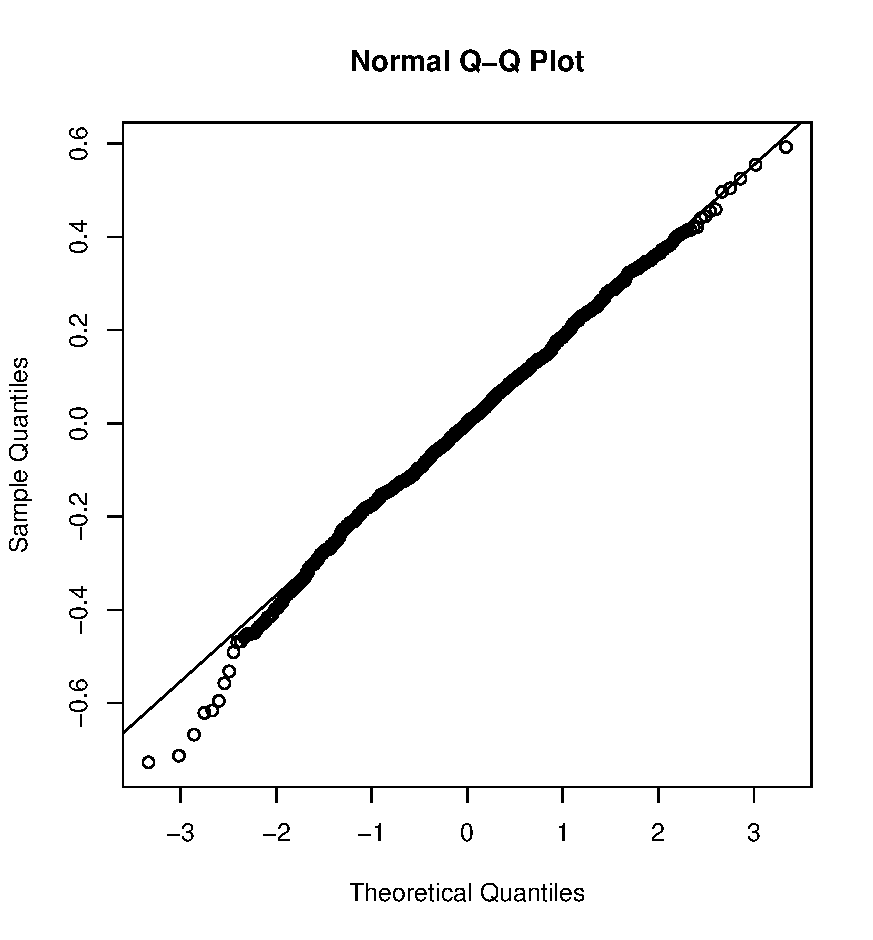
\includegraphics[width = \textwidth]{figures/denheryesyeysyes.pdf}
    \caption{Testing for normality}
    \label{fig:F_chp_resu}
\end{subfigure}%
\begin{subfigure}[b]{0.5\textwidth}
\centering
    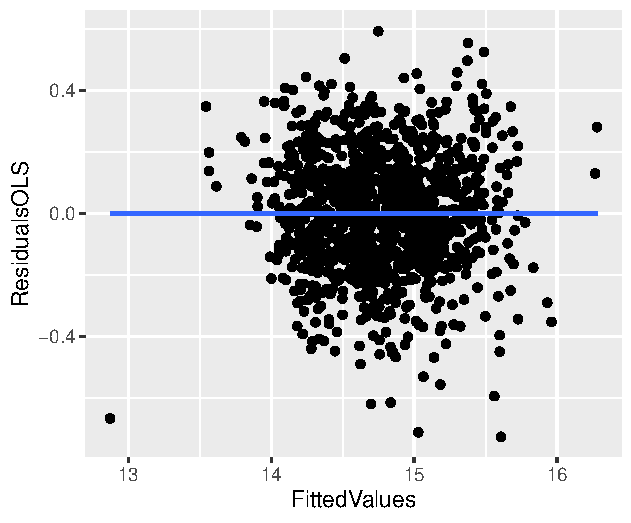
\includegraphics[width = \textwidth]{figures/RplotDenHerHejhej.pdf}
    \caption{Testing for \hetero}
    \label{fig:F_chp_hetero}
\end{subfigure}
\caption{Plots of the residuals in the linear regression performed for the model for Copenhagen determined by the F-test.}
\label{fig:F_cph_plot}
\end{figure}

From the QQ-plot in figure \ref{fig:F_chp_resu} it is seen that the residuals follow a normal distribution quite closely, wherefore we conclude the residuals satisfy assumption \ref{as:normality_of_errors}. 
From  figure \ref{fig:F_chp_hetero} we see that the residuals are randomly distributed. 
With this in mind we conclude that even though the residuals are not theoretically homoskedastic we consider for all practical purposes that the assumption is satisfied.
We therefore conclude the amount of heteroskedasticity is without substantial meaning in our tests and thus our earlier theory regarding the BLUE and hypotheses testing is valid. 
The test for heteroskedasticity has been conducted for all models found with $F$-tests and cross-validation, and has found that heteroskedasticity is theoretically present in all models but graphically that the amount of heteroskedasticity is not a concern thus we will still consider OLS as the BLUE and that hypothesis testing are still valid. 
To support this statement we will conduct both the hetero robust and usual $t$- and $F$-test for these models.

\subsubsection{Application of Heteroskedastic Robust \textit{t}-test}

In this section we wish to compare the $t$-test calculated in section \ref{ex:ttest} with the hetero robust $t$-test. 
\begin{lstlisting}
#The linear regression model, 
#which is the same as in the section with an application of t-test. 
lin_reg <-lm(log(price)~log(size),data = Copenhagen)

#Values which are the same as in the section with the application of the t-test. 
x <- c(rep(1, n), log(Copenhagen$size))
X <- matrix(data = x, nrow = n)
beta_hat <- 0.96832
beta_null <- 0
df <- n - (k + 1)

#Calculating the remaining contents of the variance formula. 
residuals <- residuals(lin_reg)
diag_residuals <- diag(lin_reg$residuals)

#Formula for variance
variance_HC <- 
    solve(t(X) %*% X) %*% t(X) %*% diag_residuals^2 %*% X %*% solve(t(X) %*% X)
    
#Square root is taken to obtain standard error
std_error_HC <- sqrt(variance_HC[2,2])

#We calculate the t-statistic
t_stat_HC <- (beta_hat-beta_null)/std_error_HC; t_stat_HC
[1] 49.05654

#p-value
p_val_HC <- pt(t_stat_HC, df = df, lower.tail = FALSE)*2; p_val_HC
[1] 4.016368e-287
\end{lstlisting}

In section \ref{ex:ttest} the $t$-value was $57.59$ and the $p$-value was $0$. 
The $t$-statistic is a bit lower with hetero robust $t$-test but the $p$-values are very similar and reach the same conclusion about our null hypothesis. 

\subsubsection{Application of Robust Heteroskedastic \textit{F}-test}
Next we will compare the hetero robust $F$-test with section \ref{sec:app_F_test}. 
\begin{lstlisting}
#First we filter the data to only contain the data for Copenhagen. 
cities.data.cph <- filter(cities.data, city == 'Copenhagen'); cities.data.cph

#The models
lin.reg1 <- lm(log(price) ~ log(size) + cond + balcony + 
    year.sale, data = cities.data)
lin.reg0 <- lm(log(price) ~ log(size) + year.sale, data = cities.data)

#Degrees of freedom and number of observations. 
df_mod1 <- n - length(lin.reg1$coefficients)
df_mod0 <- n - length(lin.reg0$coefficients)
n <- length(log(cities.data$price))
q <- df_mod0 - df_mod1

#The estimated betas found from regressing on lin.reg1
betahat <- matrix(c(10.05270, 0.99373, -0.02849, -0.16511,
    0.04648, 0.02673, 0.26932), nrow = 7, ncol = 1)

#Matrix R which checks restrictions on beta estimates for 
#cond.middel, cond.high and balcony. 
R <- matrix(c(0,0,0,0,0,0,1,0,0,0,1,0,0,0,1,0,0,0), nrow = 3, ncol = 7)

#The restrictions in R is set equal to a null vector r, 
#to see if the variables are insignificant. 
r <- matrix(c(0,0,0), nrow = 3, ncol = 1)

#The columns of X. 
intercept <- rep(1, length(cities.data.cph$price))
log.size <- log(cities.data.cph$size)
cond.medium <- ifelse(cities.data.cph$cond == 'Medium', 1, 0)
cond.high <- ifelse(cities.data.cph$cond == 'High', 1, 0)
balcony <- cities.data.cph$balcony
year.sale.crisis <- ifelse(cities.data.cph$year.sale == 'crisis', 1, 0)
year.sale.post.crisis <-
    ifelse(cities.data.cph$year.sale == 'post.crisis', 1, 0)
X <- cbind(rep(1, n), log.size, cond.medium, cond.high, 
    balcony, year.sale.crisis, year.sale.post.crisis)

#s^2 is calculated. 
resi <- rbind(lin.reg1$residuals) %*% cbind(lin.reg1$residuals)
s2 <- (  (resi)  )/(n-6-1)

#The values are insterted into the formula
#for the heteroskedastic robust F-test. 
F_wald_test <- ((   (  t(R %*% betahat - r) %*% 
    solve(R %*% solve(t(X) %*% X) %*% t(R) ) %*% 
    (R %*% betahat - r))/(q)))/s2

#The F-value and p-value from the test. 
F_value <- 22.93383
p_value_wald <- pf(q = F_wald_test, df1 = df_mod0, 
    df2 = df_mod1, lower.tail = F); 
p_value_wald
[1]    0
\end{lstlisting}

Recall the application of the $F$-test from \ref{sec:app_F_test}, where the $F$-statistic was $43.67925$ and the $p$-value was smaller than $2.2e^-16$. The $F$-statistic is much lower with the hetero robust $F$-test but the $p$-values from both tests reach the same conclusion on the null hypothesis. 




    











% The Wald statistical test on a single parameter with $\mathcal{H}_0 : \betahat_j = 0$ is given as
% \begin{align*}
%     Z_i = \dfrac{\betahat_j}{\sqrt{\Var(\betahat_j)}}
% \end{align*}
% For large $n$ the distribution is approximately $N(0,1)$. The variance $\Var(\betahat_j)$ depends on the error term and thus are invalid in the presence of heteroskedasticity.
% If we wish to test the joint significance of multiple coefficient the Wald's Statistics the test is given as
% \begin{align*}
%     W = (\mathbb{X}\betahat - \mathbf{y})^\top [\mathbf{X} \Var(\betahat) \mathbf{X}^\top](\mathbf{X}\betahat - \mathbf{y})
% \end{align*}
% This Wald Statistic is an F-statistics if it is divided with $q$. Thus o


% The asymptotic distribution of the Wald-Statistic can be used to test multiple hypotheses.




















\section{Prediction}\label{sec:prediction}
It is often wanted to deduce information about future observations based on the existing fitted regression model. 
In our case this is predicting future apartment prices. 
Due to this, prediction intervals are introduced as an estimate of an interval that contains a future observation with a certain probability with respect to already observed data.

In this section we assume a general linear model $\textbf{Y}\sim N_n(\textbf{X}\betabold, \sigma^2 \textbf{I}_n)$, where the design matrix $\textbf{X}$ has full rank $(k+1)<n$, and where $\betabold \in \mathbb{R}^{(k+1)}$ and $\sigma^2>0$ are unknown. 
Suppose an observed realization of $\textbf{Y}=\textbf{y}$ and a future random variable $Y_{n+1}$ where
\begin{align*}
    Y_{n+1}\sim N(\textbf{x}_{n+1}\betabold,\sigma^2)
\end{align*}
are independent of $\textbf{Y}$ and where $\textbf{X}$ and $\textbf{x}_{n+1}\in\mathbb{R}^{(k+1)}$ are known. 
The natural prediction value for $\textbf{Y}_{n+1}$ is the MLE for its mean, that is c.f. \eqref{eq:betahat_y}
\begin{align*}
    \hat{Y}_{n+1}(\textbf{y})=\textbf{x}_{n+1}\hat{\betabold}(\textbf{y}).
\end{align*}
The corresponding random variable $\hat{Y}_{n+1}(\textbf{Y})$ is called the predictor for $Y_{n+1}$. 
We now want to determine the variability of $Y_{n+1}$.

Given that $\hat{\betabold} \sim N_k(\betabold,\sigma^2(\textbf{X}^\top\textbf{X})^{-1})$ then $\hat{Y}_{n+1}(\textbf{Y})\sim N(\textbf{x}_{n+1}\betabold,\sigma^2\textbf{x}_{n+1}(\textbf{X}^\top\textbf{X})^{-1}\textbf{x}^\top_{n+1})$ and $Y_{n+1}\sim N(\textbf{x}_{n+1}\betabold,\sigma^2)$ are independent.
Thus we obtain uncertainty of the estimate
\begin{align*}
    Y_{n+1}-\hat{Y}_{n+1} \sim N(0, \sigma^2(1+\textbf{x}_{n+1}(\textbf{X}^\top\textbf{X})^{-1}x_{n+1}^\top)).
\end{align*}

Further the variance estimator
\begin{align*}
    s^2(\textbf{Y})=\frac{\|\textbf{Y} - \textbf{X}( \textbf{X}^\top\textbf{X} )^{-1}\textbf{X}^\top\textbf{Y}\|^2}{n-(k+1)} \sim \frac{\chi^2(n-(k+1))}{(n-(k+1))}
\end{align*}
is independent of $Y_{n+1}-\hat{Y}_{n+1}(\textbf{Y})$ because of independence of data.
From this we define
\begin{align*}
    T=\frac{Y_{n+1}-\hat{Y}_{n+1}(\textbf{Y})}{\sqrt{s^2(\textbf{Y})(1+\textbf{x}_{n+1}(\textbf{X}^\top\textbf{X})^{-1}\textbf{x}^\top_{n+1})}}
\end{align*}
and recall the proof of theorem \ref{th:t_distribution} from which we concluded that
\begin{align*}
    T=\frac{Y_{n+1}-\hat{Y}_{n+1}(\textbf{Y})/\sqrt{\sigma^2(1+\textbf{x}_{n+1}(\textbf{X}^\top\textbf{X})^{-1}\textbf{x}^\top_{n+1})}}{\sqrt{s^2(\textbf{Y})/\sigma^2}} \sim t(n-(k+1)).
\end{align*}
From this it entailes for $0<\alpha<1$ with probability $(1-\alpha)$ that $Y_{n+1}$ is contained in the interval with limits
\begin{align*}
    \hat{Y}_{n+1}(\textbf{Y})\pm t_{\alpha/2}(n-(k+1))\sqrt{s^2(\textbf{Y})(1+\textbf{x}_{n+1}(\textbf{X}^\top\textbf{X})^{-1}\textbf{x}^\top_{n+1})}
\end{align*}
and by substituting $\textbf{Y}$ with the observation $\textbf{y}$ we obtain the $(1-\alpha)\%$-prediction interval for $Y_{n+1}$
\begin{align} \label{eq:predict_interval}
    \hat{Y}_{n+1}(\textbf{y})\pm t_{\alpha/2}(n-(k+1))\sqrt{s^2(\textbf{y})(1+\textbf{x}_{n+1}(\textbf{X}^\top\textbf{X})^{-1}\textbf{x}^\top_{n+1})}
\end{align}
This is the interval of which we expect future observations to be with probability $(1-\alpha)$ given that our assumptions are correct.
If we compare the $(1-\alpha)\%$-prediction interval in \eqref{eq:predict_interval} to the $(1-\alpha)\%$-confidence interval in \eqref{eq:t_statistic} it is clear that the $(1-\alpha)\%$-prediction interval is the largest.
This is caused by prediction intervals contain both the uncertainty in estimating the ``true'' mean and the the random variation of the individual values.

\subsection{Application of Prediction}\label{subsec:app_of_prediction}
Now that we have found models based on both cross-validation and $F$-tests, we can use these models to predict 2016 apartment prices in order to validate the predictive performance of said models.
In figure \ref{fig:predictive_performance} we can see how the predictive performance differs for the two methods.
For Copenhagen the model obtained from cross-validation performs better than the model obtained using $F$-test.
However for Odense the opposite is true, here the $F$-test model performs significantly better than the one obtained from cross-validation.
As it is also evident on the plot the models found from the two methods in Aarhus and Aalborg are identical, as these have the same RMSE.
\begin{figure}[H]
    \centering
    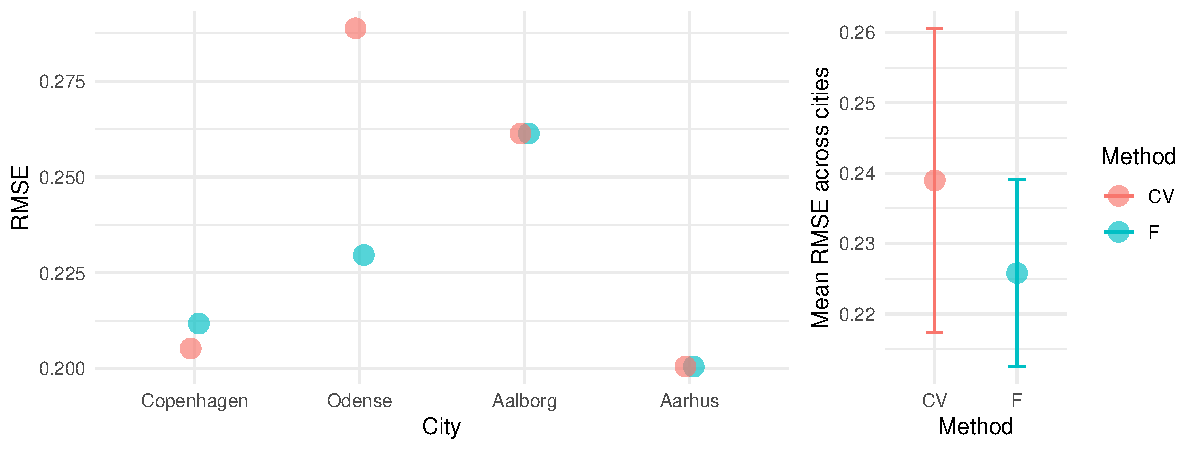
\includegraphics[width = .9\textwidth]{figures/Data_introduction/predictive_performance.pdf}
    \caption{Predicitive performance for the four cities.}
    \label{fig:predictive_performance}
\end{figure}
In table \ref{tbl:predictive_performance} the mean RMSE for the two methods across the four cities is presented.
We observe some difference between the two methods.
\begin{table}[H]
    \centering
    \begin{tabular}{lrr}
        \toprule
        \textbf{Method} & \textbf{Mean RMSE} & \textbf{RMSE std.$\!$ error}\\
        \midrule
        CV & 0.239 & 0.0216\\
        F & 0.226 & 0.0133\\
        \bottomrule
    \end{tabular}
    \caption{Mean RMSE and the associated standard error across the four cities.}
    \label{tbl:predictive_performance}
\end{table}
In our case we conclude that using $F$-test we get better slightly better predictive performance across the four cities.

\subsubsection{Prediction Interval}
We will now treat the observations from 2016 as our future observations $Y_{n+1}, \ldots, Y_{n+200}$, in order to determine if they fall inside the prediction interval.

The prediction interval is obtained using \eqref{eq:predict_interval}, or equivalently in R as
\begin{lstlisting}
    predict.int <- predict(linreg1, cities.data.2016, interval="predict")
\end{lstlisting}
Where \texttt{linreg1} is the model found in section \ref{sec:Ftest} depending on the city. 

The number of observations within this interval, for each of the models, is summed up in table \ref{tbl:Within_prediction_interval}. 
\begin{table}[H]
    \centering
    \begin{tabular}{l|rrrr}
        \toprule
        \textbf{Description} & \textbf{Copenhagen} & \textbf{Aarhus} & \textbf{Odense} & \textbf{Aalborg}\\
        \midrule
        Observations in 2016 & 108              & 46         & 27            & 19 \\
        Within Confidence Interval & 102           & 45            & 26        & 17 \\
        \% Within Confidence Interval & 94    & 98  & 96  & 89 \\
        \bottomrule
    \end{tabular}
    \caption{Observations from 2016 that fall within the prediction intervals.}
    \label{tbl:Within_prediction_interval}
\end{table}
Except for Aalborg, this seems to align well with the assumption of 95\% of observations falling within the prediction interval.
As expected from section \ref{sub:residuals} the model for Aalborg indeed has inferior predictive performance. 
While this does not verify the model, it is an indication that it can be used for prediction of future apartment prices.
These prediction intervals were found using the $F$-models, but we could just as well have used the CV-models. 
Since the models are so similar the number of observations within the prediction interval is unchanged and thus will not be repeated, see table \ref{tbl:Within_prediction_interval}.

For the dependent variable to be meaningful, it needs to be converted from $\log(price)$ back to $price$. 
This is calculated by
\begin{align*}
    price = e^{\log(price) + \frac{1}{2} s^2},
\end{align*}
since $price$ has a log-normal distribution.  
The fitted values and their prediction intervals is plotted in figure \ref{fig:predictive_intervals_observations_fitted}, along with the actual observations. 
\begin{figure}[H]
    \centering
    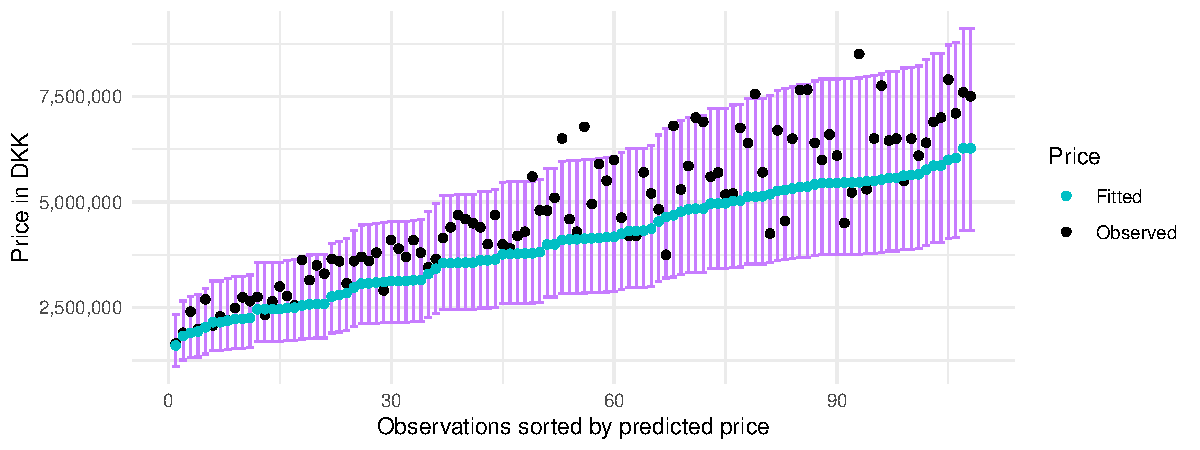
\includegraphics[width = .8\textwidth]{figures/prediction_interval.pdf}
    \caption{2016 observations for Copenhagen, fitted values and their prediction intervals.}
    \label{fig:predictive_intervals_observations_fitted}
\end{figure}
The model consistently underpredicts the price of apartments, but about 95\% still fall within the prediction intervals. 
The reason for this is likely a lacking parameter or a faulty interpretation of one or multiple of the parameters included in the model. 
This could for example be the dummy variables for year.sale. 
Here the $post.crisis$ coefficient may not be representative for the general level of house pricing in 2016.



% \begin{figure}[H]
%     \centering
%     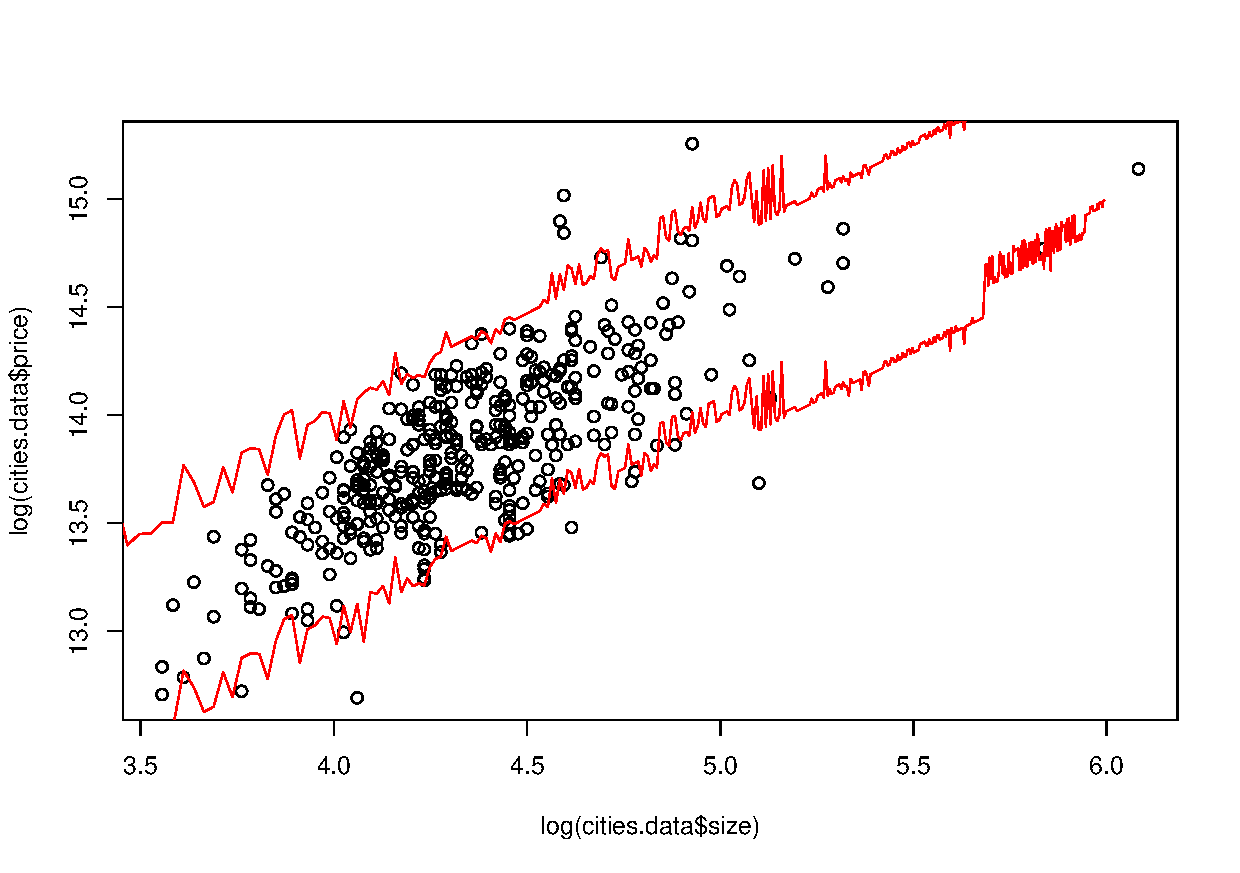
\includegraphics[width = .6\textwidth]{figures/ConfidenceInterval2015.pdf}
%     \caption{Observation for 2004-2015 and prediction interval}
%     \label{fig:confidence_intervals2015}
% \end{figure}



\section{Error Diagnostics}
In this section prediction errors of the obtained models from $F$-test and cross-validation are investigated. The investigation covers both included and previously excluded variables. We want to clarify if the errors are systematic in any way.

For Copenhagen we obtained the same model from $F$-test and cross-validation.
In figure \ref{fig:error_cont} the prediction errors of the model and the continuous predictors are plotted in scatterplots. 
Overall, the model seems to underpredict the prices on the 2016 data. 
This indicates, that the prices were generally increased in the year 2016 compared to the weighted average of the remaining years in $post.crisis$. 
The prediction errors, $pred$, seems to be heteroskedastic as the variance increases with the size of the predicted values. 
This might indicates some unexplained structure in the errors or could just be caused by randomness. 
$selling.period$ and $year.construct$, which were excluded from the model, only have a small negative slope and therefore would not contribute with much explanatory value for the 2016 data.
The errors of $size$ appear heteroskedastic as the variance peeks at the middle. 
\begin{figure}[H]
        \centering
      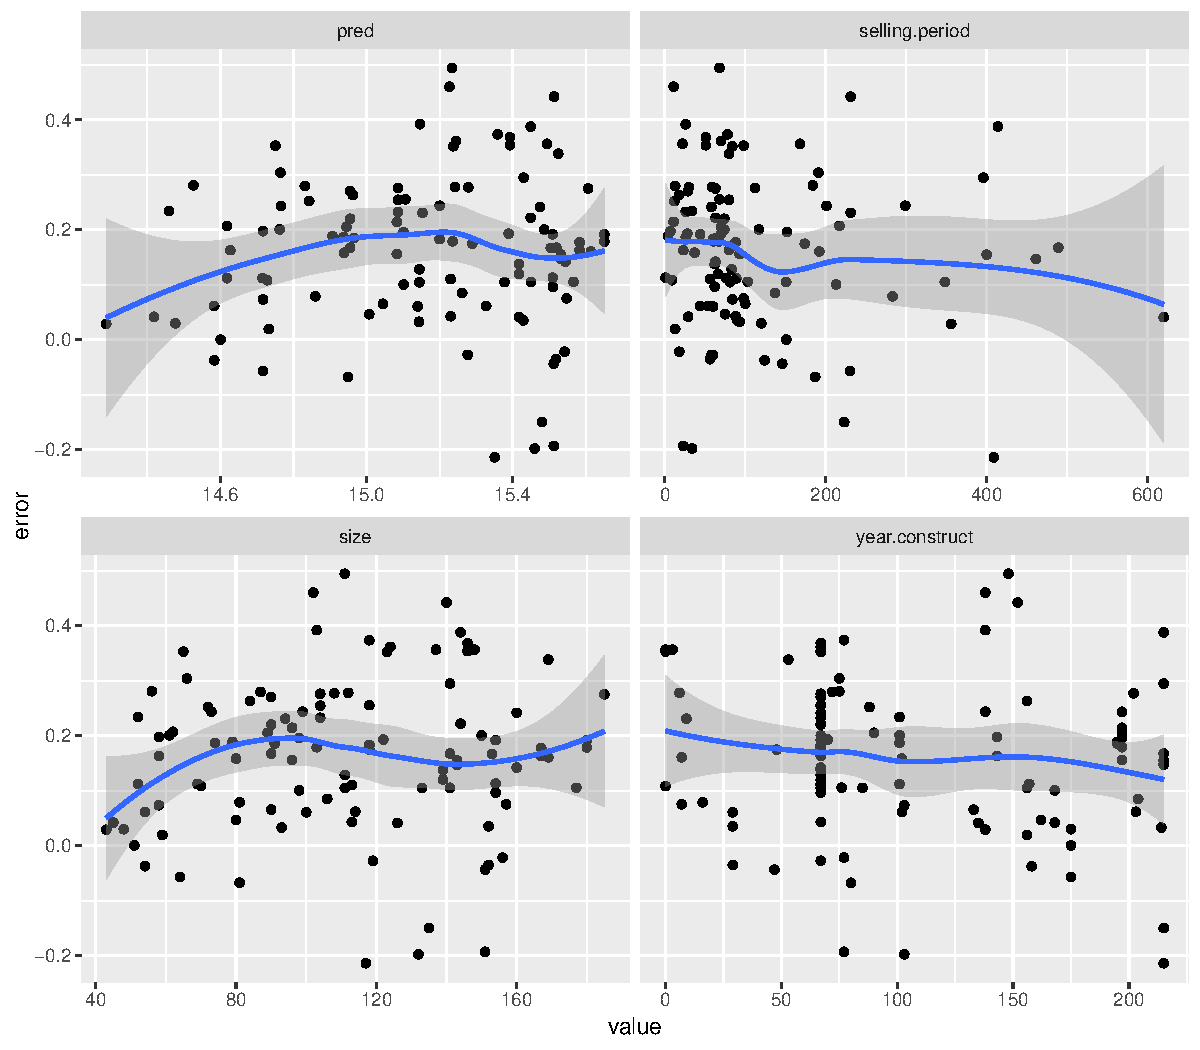
\includegraphics[width = 0.7 \textwidth]{figures/Nanna/errors_continuous.pdf}
      \caption{Scatterplots of the prediction errors calculated from the model found for Copenhagen. }
      \label{fig:error_cont}
\end{figure}
In figure \ref{fig:error_factor} are boxplots of the factor variables. 
Again, an overall conclusion is, that the model underpredicts the data from 2016.
For $balcony$ the median is almost the same for each of the two values.
However, the distribution of the errors of apartments with $balcony$ is skewed and has potential outliers. 
For $cond$ the errors decreases with the state of the condition of the apartments.
The value ``Low'' is affected by a small number of observations. 
\textit{renovation}, which was excluded from the model, has almost the same median error for each of its two values. 
\begin{figure}[H]
        \centering
      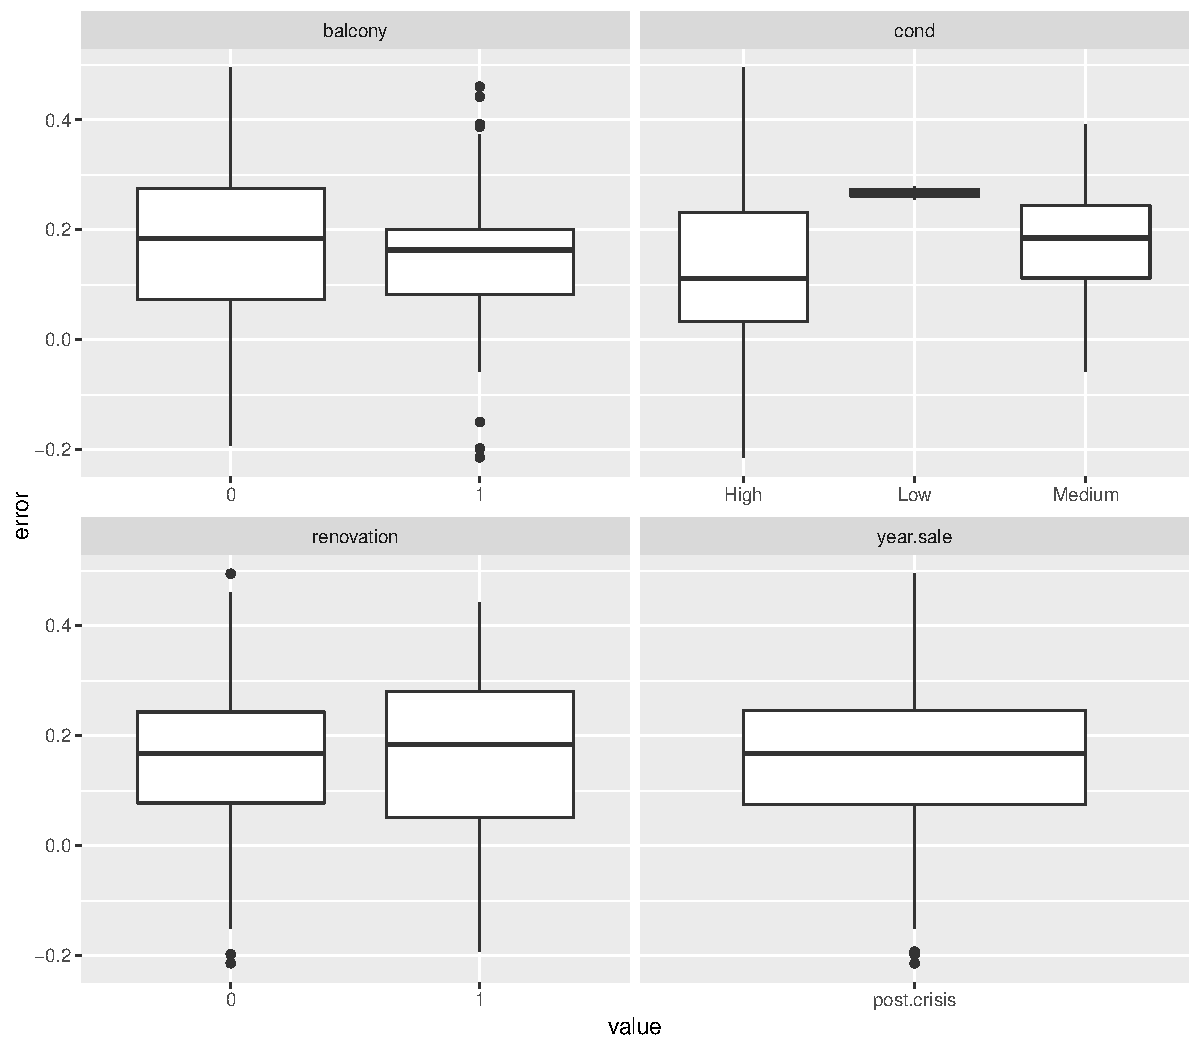
\includegraphics[width = 0.7 \textwidth]{figures/Nanna/errors_factors.pdf}
      \caption{Boxplots of the prediction errors calculated from the model found for Copenhagen.}
      \label{fig:error_factor}
\end{figure}
A lot of the same conclusions are drawn about the remaining models and all the models underpredict the prices due to the majority of the errors being positive.
The models obtained from F-test and cross-validation only differs for Aarhus and Odense, but these have very similar prediction errors.
All the models underpredict the prices due to the majority of the errors being positive.
$renovation$ seems to be able to add some explanatory value to the 2016 data for the models for Aarhus and Odense.  
The relation between prediction errors and $cond$ is a little different between cities. 

From the error diagnostic the main conclusion is that the models underpredict.
This is to a great extent caused by the omission of the increasing trend in prices in the $post.crisis$ category. 